\documentclass[11pt]{article}
\usepackage[margin=0.7in]{geometry}
\usepackage[T1]{fontenc}
\usepackage{lmodern}
\usepackage{amsmath,amssymb}
\usepackage{booktabs,longtable,array}
\usepackage{graphicx}
\usepackage[colorlinks=true,linkcolor=blue,citecolor=blue,urlcolor=blue]{hyperref}

\newcommand{\repourl}{https://github.com/Barghav777/SCWR_3D}
\graphicspath{{graphs/}{../figures/}{./}}
\setlength{\emergencystretch}{3em}
\setlength{\textfloatsep}{8pt plus 2pt minus 2pt}
\setlength{\floatsep}{6pt plus 2pt minus 2pt}
\setlength{\intextsep}{6pt plus 2pt minus 2pt}
\renewcommand{\topfraction}{0.95}
\renewcommand{\bottomfraction}{0.90}
\renewcommand{\textfraction}{0.05}
\renewcommand{\floatpagefraction}{0.88}
\renewcommand{\arraystretch}{1.15}
\sloppy

\title{\textbf{Case-disjoint benchmark of surrogate models for flow and thermal fields in supercritical $\mathrm{CO}_2$ natural-circulation loops}}
\author{}
\date{}

\begin{document}
\maketitle

\begin{abstract}
Surrogate models for supercritical carbon dioxide ($\mathrm{sCO}_2$) natural-circulation loops (NCLs) can replace day-long steady-state conjugate computational fluid dynamics (CFD) simulations with millisecond-scale field predictions, yet most published evaluations rely on random node-level train--test splits or single pooled metrics that mask generalization failure across unseen operating conditions. Here we present a case-disjoint surrogate benchmark built from 42 steady-state RANS simulations solved with a $k$--$\varepsilon$ family turbulence model ($k$ and $\varepsilon$ are exported) and a Span--Wagner equation of state verified against \texttt{CoolProp} (median $0.0008\%$) across three heater--cooler configurations (\texttt{HHHC}, \texttt{HHVC}, and \texttt{VHVC}) and two loop scales. Across three random seeds, we benchmark 17 surrogate models (plus an input-concatenation conditioning ablation) spanning tree ensembles, Fourier-coordinate neural networks, physics-informed neural networks (PINNs), DeepONet, Latent Neural Operator, Transolver-style attention, multi-scale graph networks, Fourier neural operators (\texttt{F-FNO}, \texttt{U-FNO}), and proper orthogonal decomposition (\texttt{POD}) reduced-order models under five-fold stratified case-disjoint cross-validation and leave-one-group-out extrapolation. We show that random node splitting understates five-fold case-disjoint error across the four nonlinear tree baselines by roughly an order of magnitude on thermodynamic state fields ($6.78\times\text{--}10.37\times$ on density, $11.29\times\text{--}87.54\times$ on gauge pressure, and $5.62\times\text{--}10.24\times$ on temperature in case-macro MAE) because high-capacity models memorize case-specific operating levels from adjacent mesh nodes. We also show that separating closed-loop gauge pressure into its case-level thermal-pressurization offset and centered spatial residual prevents small within-case hydrostatic variations from distorting model rankings. Across the eight exported CFD fields, no single architecture wins universally: among cross-configuration pooled models, \texttt{DeepONet} and \texttt{PINN continuity} lead on density and temperature, \texttt{Extra Trees} best predicts case-level gauge pressure, and multiplicative feature-modulated coordinates (\texttt{Domain-informed FiLM-MLP}) achieve the lowest error across both turbulence fields ($k, \varepsilon$) and all three velocity components ($u, v, w$), while within-group \texttt{POD-RBF} yields the sharpest temperature and turbulence reconstructions when interpolating on a fixed loop mesh.
\end{abstract}

\medskip\noindent\textbf{Keywords:} supercritical $\mathrm{CO}_2$, natural-circulation loop, CFD surrogate benchmark, case-disjoint validation, neural operators, proper orthogonal decomposition

\section{Introduction}
Natural-circulation loops (NCLs) operating with supercritical fluids remove heat without mechanical pumps by balancing buoyancy forces between heated and cooled sections against frictional and local losses~\cite{swapnalee2012generalized,vijayan2002experimental,pioro2007heat}. Supercritical carbon dioxide ($\mathrm{sCO}_2$, critical point $T_c = 304.13\text{ K} = 30.98^\circ\text{C}$, $p_c = 7.3773\text{ MPa} = 73.773\text{ bar}$) is widely used as a scaled simulant fluid for supercritical water reactor (SCWR) thermal-hydraulics and compact power cycles because its lower critical point permits experiments and conjugate CFD studies near the pseudocritical locus~\cite{span1996new,dostal2004supercritical,bae2005mixed}. Near the pseudocritical temperature, steep variations in density $\rho$, specific heat $c_p$, viscosity $\mu$, and thermal conductivity $k$ strongly couple buoyancy gradients with turbulence production and heat transfer~\cite{kurganov2013heat,sarkar2014entropy,chen2013numerical}.

Because resolving conjugate heat transfer between the primary $\mathrm{sCO}_2$ pipe, the solid metallic wall, and the secondary cooling-water jacket requires fine near-wall meshes and real-gas property evaluations, each steady-state RANS simulation in our dataset requires roughly 24 hours of compute time. Data-driven spatial surrogates---including gradient-boosted trees~\cite{friedman2001greedy,chen2016xgboost,prokhorenkova2018catboost}, coordinate neural networks~\cite{raissi2019physics,tancik2020fourier,perez2018film}, neural operators~\cite{lu2021learning,li2021fourier,wen2022ufno,wu2024transolver}, and proper orthogonal decomposition (POD) reduced-order models~\cite{berkooz1993proper,audouze2009nonintrusive}---provide millisecond-scale predictions once trained. However, three practical issues complicate surrogate benchmarking on closed natural-circulation loops: (i) random node-level train--test splits leak case-specific operating levels across neighboring mesh nodes; (ii) pooled metrics such as $R^2$ conflate between-case operating-level shifts with within-case spatial profile accuracy, while naive within-case normalization breaks down for gauge pressure in closed loops; and (iii) slender circular pipes ($D_i/L \sim 10^{-2}$) and varying heater--cooler orientations create different inductive-bias requirements for thermodynamic state fields versus velocity and turbulence fields.

To address these issues, this paper contributes: (1) a controlled comparison of 80/20 random-node splitting against five-fold case-disjoint cross-validation across four nonlinear tree models and two linear/constant controls; (2) a physical characterization and two-part evaluation protocol for closed-loop gauge pressure; and (3) a three-seed benchmark of 18 surrogate model variants across eight CFD fields under both five-fold case-disjoint interpolation and leave-one-group-out geometric extrapolation.

\section{Physical Domain and $\mathrm{sCO}_2$ Natural-Circulation Loop Dataset}
\subsection{Loop Geometry, CFD Solver Configuration, and Primary Fluid Domain}
The dataset consists of 42 converged steady-state RANS conjugate heat-transfer simulations of closed rectangular $\mathrm{sCO}_2$ natural-circulation loops solved in ANSYS Fluent and exported on cross-sectional planes via ANSYS CFD-Post. All simulations use a $k$--$\varepsilon$ family turbulence model ($k$ and $\varepsilon$ are exported) and a Span--Wagner equation of state verified against \texttt{CoolProp}~\cite{span1996new,bell2014pure} (median relative density discrepancy $0.0008\%$) for the primary $\mathrm{sCO}_2$ fluid.

The 42 cases cover three heater--cooler configurations---horizontal heater/horizontal cooler (\texttt{HHHC}), horizontal heater/vertical cooler (\texttt{HHVC}), and vertical heater/vertical cooler (\texttt{VHVC})---across two loop scales (Table~\ref{tab:dataset}): 29 small-loop cases ($L_x \times L_y = 0.8936 \times 1.0000\text{ m}$, $D_i = 15.00\text{ mm}$) and 13 large-loop \texttt{VHVC} cases ($L_x \times L_y = 3.0100 \times 4.0800\text{ m}$, $D_i = 13.84\text{ mm}$). Complete radial dimensions of the stainless-steel wall and cooling-water jacket, axial heater/cooler spans, and sampling-plane counts (97 planes in small loops; 142 planes in the large loop) are given in Supplementary Section~S1.

Each simulation is defined by four boundary parameters encoded in its case name \texttt{\{CONFIG\}\_P\{Q\}\_\{p\}\_bar\_\{mdot\}kgs\_T\_\{Tin\}}: heater power $Q \in [10, 2500]\text{ W}$, operating pressure $p_{\mathrm{op}} \in \{80, 85, 90, 100\}\text{ bar}$, cooling-water mass flow rate $\dot{m} \in [0.010, 0.150]\text{ kg s}^{-1}$, and cooling-water inlet temperature $T_{\mathrm{in}} \in \{283.5, 300, 305, 315\}\text{ K}$ (Fig.~\ref{fig:pairplot}). At each node $(x,y,z)$, eight CFD target fields are exported: density $\rho\text{ (kg m}^{-3}\text{)}$, gauge pressure $p_{\mathrm{gauge}}\text{ (Pa)}$, temperature $T\text{ (}^\circ\text{C)}$, turbulence eddy dissipation $\varepsilon\text{ (m}^2\text{ s}^{-3}\text{)}$, turbulence kinetic energy $k\text{ (m}^2\text{ s}^{-2}\text{)}$, and velocity components $(u,v,w)\text{ (m s}^{-1}\text{)}$. Removing solid wall nodes (\texttt{null} velocity/turbulence, $\rho \approx 7970\text{ kg m}^{-3}$) and outer cooling-water jacket nodes ($\rho > 950\text{ kg m}^{-3}$) and deduplicating intersecting plane coordinates yields $5,451,341$ unique primary $\mathrm{sCO}_2$ nodes ($\rho \in [153.2, 892.5]\text{ kg m}^{-3}$; Fig.~\ref{fig:distributions}).

\begin{table}[!htbp]
\centering
\caption{Summary of the 42 steady-state CFD cases by heater--cooler configuration and loop scale. Full radial and plane-sampling details are in Supplementary Section~S1.}
\label{tab:dataset}
\small
\setlength{\tabcolsep}{4.8pt}
\begin{tabular}{llccccrrr}
\toprule
Config. & Scale & Cases & $L_x \times L_y$ (m) & $D_i$ (mm) & $Q$ (W) & $p_{\mathrm{op}}$ (bar) & $\dot{m}$ (kg s$^{-1}$) & $\mathrm{sCO}_2$ nodes/case \\
\midrule
\texttt{HHHC} & Small & 20 & $0.894 \times 1.000$ & 15.00 & 1000--2000 & 80--100 & 0.050--0.150 & 97,264 \\
\texttt{HHVC} & Small & 5  & $0.894 \times 1.000$ & 15.00 & 10--50     & 90      & 0.050        & 89,771 \\
\texttt{VHVC} & Small & 4  & $0.894 \times 1.000$ & 15.00 & 10--40     & 90      & 0.050        & 89,647 \\
\texttt{VHVC} & Large & 13 & $3.010 \times 4.080$ & 13.84 & 250--2500  & 85      & 0.010--0.035 & 207,586 \\
\midrule
\textbf{Total} & \textbf{4 groups} & \textbf{42} & -- & -- & \textbf{10--2500} & \textbf{80--100} & \textbf{0.010--0.150} & \textbf{5,451,341 total} \\
\bottomrule
\end{tabular}
\end{table}

\begin{figure}[!htbp]
\centering
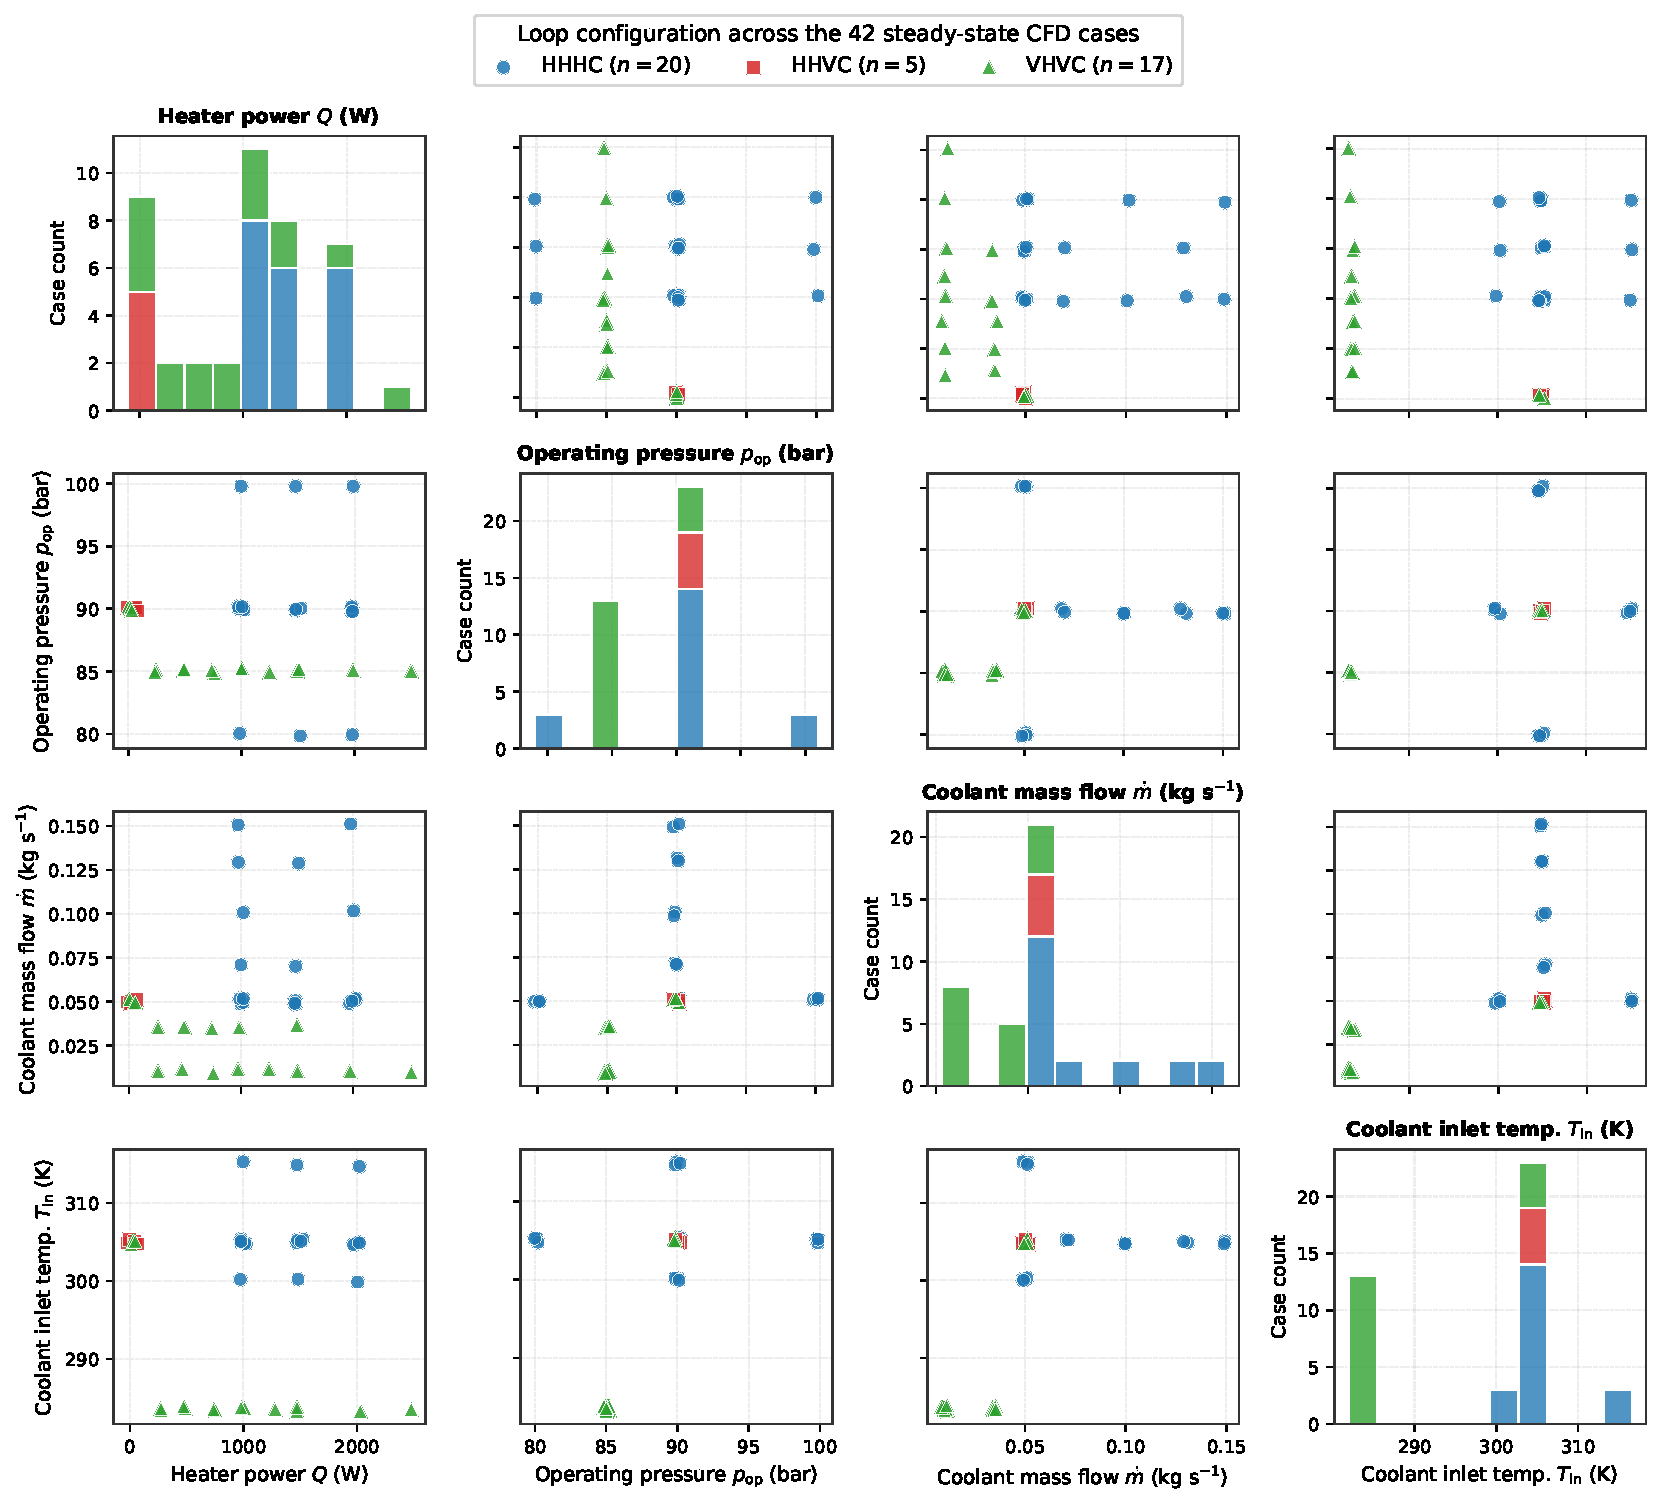
\includegraphics[width=0.98\textwidth]{operating_condition_pairplot_by_configuration.pdf}
\caption{Operating-condition distribution across the 42 steady-state CFD cases by heater--cooler configuration (\texttt{HHHC}, \texttt{HHVC}, \texttt{VHVC}). Diagonal panels show stacked case-count histograms for $Q$, $p_{\mathrm{op}}$, $\dot{m}$, and $T_{\mathrm{in}}$.}
\label{fig:pairplot}
\end{figure}

\begin{figure}[!htbp]
\centering
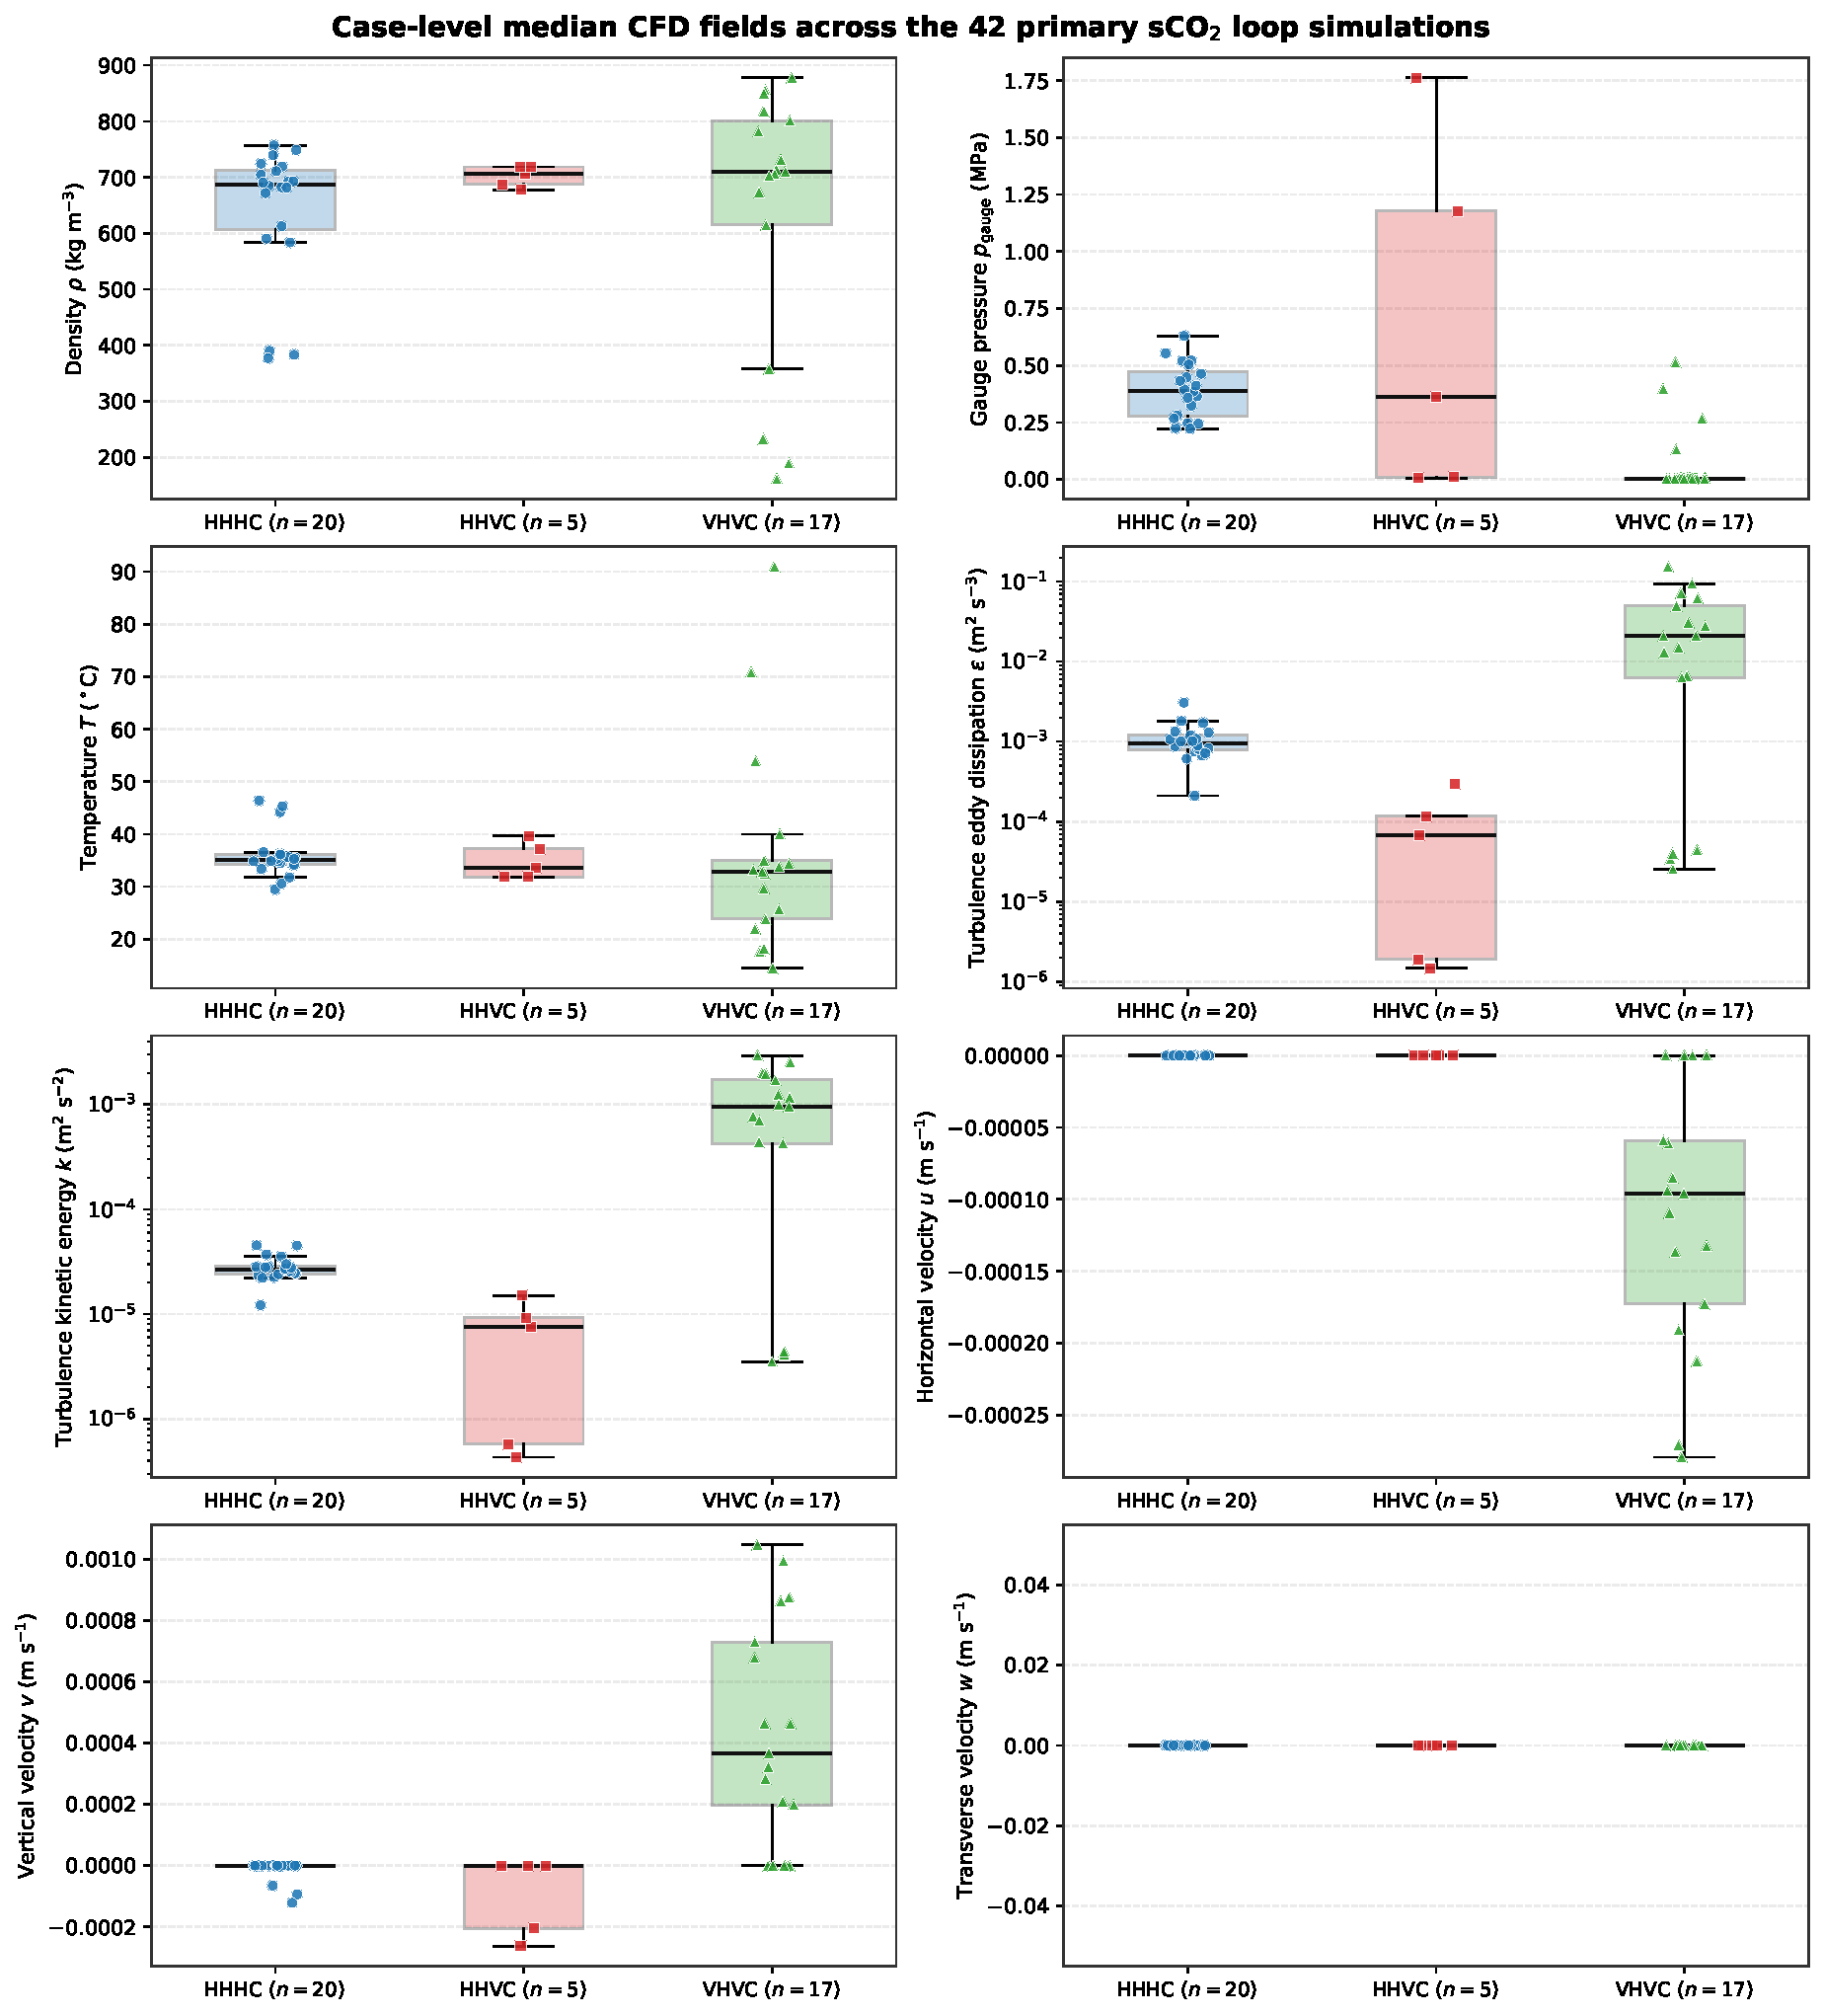
\includegraphics[width=0.98\textwidth]{case_median_target_distributions_co2_candidate.pdf}
\caption{Case-level median distributions of the eight exported CFD fields across the 42 primary $\mathrm{sCO}_2$ loop simulations ($5,451,341$ nodes), grouped by configuration (\texttt{HHHC}, \texttt{HHVC}, \texttt{VHVC}).}
\label{fig:distributions}
\end{figure}

\subsection{Behavior of Exported Gauge Pressure Across Cases}
In all 42 simulations, the local absolute pressure used to evaluate $\mathrm{CO}_2$ properties is the sum of the operating pressure $p_{\mathrm{op}}$ and the exported gauge pressure $p_{\mathrm{gauge}}(\mathbf{x})$:
\begin{equation}
  p_{\mathrm{abs}}(\mathbf{x}) = p_{\mathrm{op}} + p_{\mathrm{gauge}}(\mathbf{x}).
  \label{eq:piezometric}
\end{equation}
Evaluating $(T(\mathbf{x}), p_{\mathrm{abs}}(\mathbf{x}))$ in \texttt{CoolProp}~\cite{span1996new,bell2014pure} matches the exported CFD density $\rho(\mathbf{x})$ across all 42 cases to a median relative difference of $0.0008\%$ ($0.00004\%\text{--}0.0015\%$). Within any single case $c$, $p_{\mathrm{gauge}}$ varies very little around the loop because the solver subtracts a constant reference hydrostatic head: the within-case standard deviation $\sigma_c(p_{\mathrm{gauge}})$ is only $0.15\text{--}0.39\text{ kPa}$ in the small loops and $1.45\text{--}8.79\text{ kPa}$ in the large loop (42-case mean $\bar{\sigma}_c = 1.51\text{ kPa}$).

Across different cases, however, the case-mean gauge pressure $\bar{p}_c$ spans $1.42\text{ kPa}$ to $1.763\text{ MPa}$ (Fig.~\ref{fig:pressure}):
\begin{itemize}
  \item \textbf{Large loop vs.\ small loops:} In the 13 large-loop \texttt{VHVC} cases, the reference gauge pressure is pinned near $0\text{ Pa}$ at the top of the loop ($y = 4.08\text{ m}$), keeping $\bar{p}_c \in [1.42, 8.77]\text{ kPa}$ (Fig.~\ref{fig:pressure}a). In the 29 small-loop cases (\texttt{HHHC}, \texttt{HHVC}, and small \texttt{VHVC}), the closed fluid domain has no pressure-outlet pin, so $\bar{p}_c$ rises with the loop-mean temperature $\bar{T}_c$.
  \item \textbf{Empirical pressure--temperature slope vs.\ \texttt{CoolProp}:} Across the 17 small-loop cases at $p_{\mathrm{op}} = 90\text{ bar}$ and $T_{\mathrm{in}} = 305\text{ K}$, a linear fit of $\bar{p}_c$ versus $\bar{T}_c$ gives an \emph{empirical slope} of $0.214\text{ MPa K}^{-1}$ ($0.235\text{ MPa K}^{-1}$, or $\approx 0.23\text{ MPa K}^{-1}$, across the five \texttt{HHVC} cases; Fig.~\ref{fig:pressure}b). By comparison, the theoretical constant-density derivative $(\partial p/\partial T)_\rho$ computed in \texttt{CoolProp} at each case's mean density and temperature is $0.315\text{--}0.365\text{ MPa K}^{-1}$ (median $0.338\text{ MPa K}^{-1}$, or $\approx 0.35\text{ MPa K}^{-1}$ near $\rho = 710\text{ kg m}^{-3}$ and $T = 305\text{--}308\text{ K}$; $0.133\text{--}0.417\text{ MPa K}^{-1}$ across all 29 small-loop cases in Supplementary Table~S0b). Testing the fixed-mass hypothesis via the plane-weighted mean $\mathrm{CO}_2$ density $\bar{\rho}_{\mathrm{plane},c}$ across cases at the same $(p_{\mathrm{op}}, T_{\mathrm{in}})$ shows that $\bar{\rho}_{\mathrm{plane},c}$ is not strictly constant: at $90\text{ bar}, 305\text{ K}$ it spans $671.6\text{--}704.0\text{ kg m}^{-3}$ ($\mathrm{SD}=9.79\text{ kg m}^{-3}$) in \texttt{HHHC}, $681.2\text{--}717.8\text{ kg m}^{-3}$ ($\mathrm{SD}=16.66\text{ kg m}^{-3}$) in \texttt{HHVC}, and $696.8\text{--}712.1\text{ kg m}^{-3}$ ($\mathrm{SD}=6.62\text{ kg m}^{-3}$) in small \texttt{VHVC} (and $161.5\text{--}860.8\text{ kg m}^{-3}$, $\mathrm{SD}=270.83\text{ kg m}^{-3}$ in top-pinned \texttt{VHVC/large}). Because $\bar{\rho}_{\mathrm{plane},c}$ decreases slightly in warmer cases ($\mathrm{d}\bar{\rho}/\mathrm{d}\bar{T} < 0$), the relation $\mathrm{d}\bar{p} \approx (\partial p/\partial T)_\rho\,\mathrm{d}\bar{T} + (\partial p/\partial \rho)_T\,\mathrm{d}\bar{\rho}$ yields an empirical slope lower than the constant-density \texttt{CoolProp} value.
  \item \textbf{Near-stagnant steady solutions in \texttt{HHVC} at $20\text{ W}$ and $30\text{ W}$:} In the five \texttt{HHVC} cases at $90\text{ bar}$ and $305\text{ K}$, the $Q = 20\text{ W}$ and $30\text{ W}$ runs (\texttt{HHVC\_P20\_90\_bar\_0.05kgs\_T\_305} and \texttt{HHVC\_P30\_90\_bar\_0.05kgs\_T\_305}) are near-stagnant steady solutions (mean speed $\overline{|\mathbf{u}|} = 0.9\text{--}1.1\text{ mm s}^{-1}$, $\bar{T}_c = 31.92\text{--}31.94^\circ\text{C}$, $\bar{p}_c = 6.1\text{--}9.2\text{ kPa}$), whereas the $10\text{ W}$, $40\text{ W}$, and $50\text{ W}$ runs have sustained buoyant circulation ($\overline{|\mathbf{u}|} = 0.044\text{--}0.107\text{ m s}^{-1}$, $\bar{T}_c = 33.58\text{--}39.36^\circ\text{C}$, $\bar{p}_c = 0.361\text{--}1.763\text{ MPa}$; Fig.~\ref{fig:pressure}b).
\end{itemize}

\begin{figure}[!htbp]
\centering
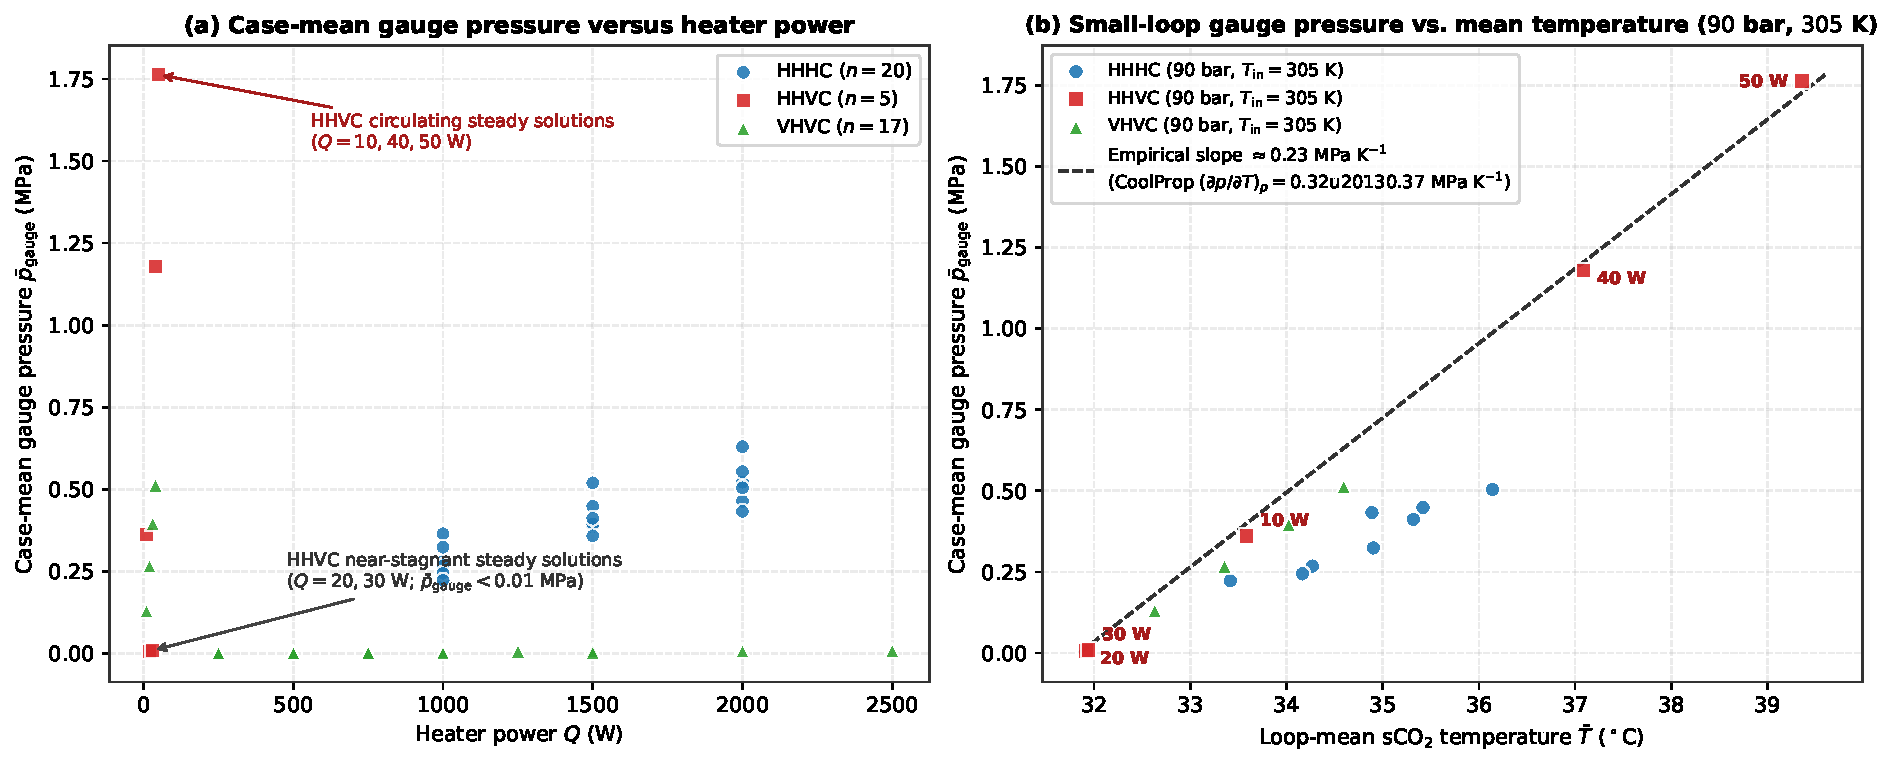
\includegraphics[width=1.00\textwidth]{co2_candidate_case_mean_gauge_pressure_vs_power.pdf}
\caption{Case-level gauge-pressure behavior across the 42 $\mathrm{sCO}_2$ simulations. (a) Case-mean gauge pressure $\bar{p}_{\mathrm{gauge}}$ versus heater power $Q$. (b) In the 17 small-loop cases at $p_{\mathrm{op}}=90\text{ bar}$ and $T_{\mathrm{in}}=305\text{ K}$, $\bar{p}_{\mathrm{gauge}}$ follows an empirical slope of $0.214\text{ MPa K}^{-1}$ ($0.235\text{ MPa K}^{-1}$ across \texttt{HHVC}) versus loop-mean temperature $\bar{T}_c$, compared against the \texttt{CoolProp} constant-density derivative $(\partial p/\partial T)_\rho = 0.315\text{--}0.365\text{ MPa K}^{-1}$ (median $0.338\text{ MPa K}^{-1}$).}
\label{fig:pressure}
\end{figure}

\section{Benchmark Methodology, Models, and Evaluation Protocol}
\subsection{Validation Protocols and Evaluation Metrics}
Every model predicts the eight target fields $\mathbf{y}(\mathbf{x}, \mathbf{c}) \in \mathbb{R}^8$ at coordinates $\mathbf{x} = (x,y,z)$ given the case descriptor $\mathbf{c} = (Q, p_{\mathrm{op}}, \dot{m}, T_{\mathrm{in}}, L_x, L_y, D_i, \text{one-hot config})$. We evaluate three validation protocols:
\begin{enumerate}
  \item \textbf{Five-fold stratified case-disjoint cross-validation:} For each seed $s \in \{2026, 2027, 2028\}$, the 42 cases are split into five folds ($9, 9, 8, 8, 8$ cases) stratified by the four groups (\texttt{HHHC/small}, \texttt{HHVC/small}, \texttt{VHVC/small}, \texttt{VHVC/large}). Each seed independently re-randomizes the five-fold case partition, the four validation cases per fold, the training node subsample ($30,000$ nodes/case in GPU 3-seed CV; $20,000$ in the CPU split test), and model initialization. Held-out test cases are evaluated on 100\% of their mesh nodes ($5,451,341$ out-of-fold predictions per seed).
  \item \textbf{Within-group mesh-aligned cross-validation:} Mesh-aligned models (\texttt{POD-RBF}, \texttt{POD-GPR}, \texttt{Nearest case}) require a shared mesh ordering and therefore train and predict strictly within the matching configuration/scale group of each five-fold split.
  \item \textbf{Leave-one-group-out extrapolation:} All cases in one structural group (\texttt{HHHC/small}, $n=20$; \texttt{HHVC/small}, $n=5$; \texttt{VHVC/small}, $n=4$; or \texttt{VHVC/large}, $n=13$) are held out while the 16 cross-configuration pooled models train on the remaining three groups ($16\text{ models} \times 8\text{ fields} = 128$ model--field evaluations per group).
\end{enumerate}

For each held-out case $c$ ($N_c$ nodes, truth $y_{c,i}$, prediction $\hat{y}_{c,i}$, within-case standard deviation $\sigma_c$), we compute case-level MAE, RMSE, case-normalized MAE ($\mathrm{nMAE}_c = \mathrm{MAE}_c / \sigma_c$), and node-pooled $R^2_{\mathrm{pooled}}$:
\begin{equation}
  \mathrm{MAE}_c = \frac{1}{N_c}\sum_{i=1}^{N_c} |\hat{y}_{c,i} - y_{c,i}|, \quad
  \mathrm{RMSE}_c = \sqrt{\frac{1}{N_c}\sum_{i=1}^{N_c} (\hat{y}_{c,i} - y_{c,i})^2}, \quad
  R^2_{\mathrm{pooled}} = 1 - \frac{\sum_{c,i}(\hat{y}_{c,i} - y_{c,i})^2}{\sum_{c,i}(y_{c,i} - \bar{y}_{\mathrm{all}})^2}.
\end{equation}
Across the 42 cases, we report case-macro MAE, case-macro RMSE, median case nMAE, and $R^2_{\mathrm{pooled}}$. Because $\bar{\sigma}_c(p_{\mathrm{gauge}}) = 1.51\text{ kPa}$ is small relative to between-case pressure shifts (Section~2.2), we suppress raw $\mathrm{nMAE}_c$ for $p_{\mathrm{gauge}}$ and evaluate the case-mean level error $e_{\mathrm{level},c}$ and centered spatial residual $\tilde{p}_{c,i} = p_{c,i} - \bar{p}_c$ separately:
\begin{equation}
  e_{\mathrm{level},c} = |\hat{\bar{p}}_c - \bar{p}_c|, \quad
  \mathrm{RMSE}_{\mathrm{res},c} = \sqrt{\frac{1}{N_c}\sum_{i=1}^{N_c}\bigl(\tilde{\hat{p}}_{c,i} - \tilde{p}_{c,i}\bigr)^2}, \quad
  \mathrm{nRMSE}_{\mathrm{res},c} = \frac{\mathrm{RMSE}_{\mathrm{res},c}}{\max(\sigma_c, 1\text{ kPa})}.
\end{equation}

\subsection{Benchmark Model Suite and Verified Hyperparameters}
Table~\ref{tab:models} summarizes all evaluated models, their conditioning mechanisms, and their verified hyperparameters from \texttt{notebooks/kaggle\_clean\_case\_cv\_predictions.ipynb} and \texttt{scripts/cpu\_clean\_benchmarks.py}. To isolate multiplicative feature modulation in coordinate networks, \texttt{Domain-informed FiLM-MLP} modulates each hidden block by $\mathbf{h}^{(\ell)} \odot (1 + \boldsymbol{\gamma}^{(\ell)}(\mathbf{c})) + \boldsymbol{\beta}^{(\ell)}(\mathbf{c})$~\cite{perez2018film}, whereas its matched ablation \texttt{Domain-informed Concat-MLP} concatenates $\mathbf{c}$ at the input layer.

\begin{table}[!htbp]
\centering
\caption{Evaluated surrogate models, spatial representations, and verified hyperparameters.}
\label{tab:models}
\footnotesize
\setlength{\tabcolsep}{4.5pt}
\begin{tabular}{p{3.4cm}p{2.3cm}p{10.5cm}}
\toprule
Model & Family & Conditioning representation \& verified hyperparameters \\
\midrule
\texttt{Mean baseline} & Constant & Predicts training-fold node mean per target field. \\
\texttt{Ridge} & Linear & $\ell_2$ linear regression ($\alpha=10.0$) on standardized $[\mathbf{x},\mathbf{c}]$. \\
\texttt{Random Forest} & Bagged trees & Multi-output CART on $[\mathbf{x},\mathbf{c}]$: 48 trees (80 in CPU split test), max depth 20, max leaf nodes 4096 (2048 CPU), min leaf 5, max features $0.8$, bootstrap $0.3$. \\
\texttt{Extra Trees} & Random trees & Multi-output randomized trees on $[\mathbf{x},\mathbf{c}]$: 64 trees (96 CPU), depth 20, max leaf 4096. \\
\texttt{XGBoost} & Boosted trees & Per-target \texttt{hist} trees: 300 trees (220 CPU), depth 8 (6 random-node CPU), lr $0.08$, subsample $0.85$, colsample $0.85$, $\lambda=2.0$. \\
\texttt{CatBoost} & Oblivious trees & Multi-output symmetric trees (\texttt{MultiRMSE}): 350 iterations, depth 8, lr $0.08$, $\ell_2=3.0$. \\
\texttt{DeepONet} & Operator net & 4-layer branch MLP on $\mathbf{c}$ + 4-layer trunk MLP on $\mathbf{x}$ (width 256, latent 128), MSE loss, AdamW ($\text{lr}=5\times 10^{-4}$), batch 8192 ($8\text{ min}$ cap/fold). \\
\texttt{PINN data-only} & Coord.\ MLP & 5-layer Fourier-coordinate MLP ($B=4$ bands, width 256, GELU + LayerNorm), MSE loss. \\
\texttt{PINN continuity} & Physics MLP & Identical to \texttt{PINN data-only} + $\lambda_{\mathrm{cont}}=0.05\|\nabla\cdot(\hat{\rho}\hat{\mathbf{u}})\|_2^2$ on 1024 collocation nodes/step. \\
\texttt{Domain-informed FiLM-MLP} & Modulated MLP & 5-block residual MLP (width 256, $B=4$ Fourier bands + leg centerline/arc-length features), FiLM modulation by $\mathbf{c}$, Huber loss ($\delta=1.0$), AdamW ($\text{lr}=5\times 10^{-4}$, batch 8192). \\
\texttt{Domain-informed Concat-MLP} & Ablation MLP & Identical architecture and training to \texttt{FiLM-MLP}, but concatenates $\mathbf{c}$ at the input layer. \\
\texttt{Latent Neural Operator} & Latent attn. & Cross-attention from Fourier coordinates ($B=4$) to $M=24$ latent tokens (width 128, 4 heads, branch/query depth 3, decoder depth 2), Huber loss. \\
\texttt{Transolver-style} & Slice attn. & 4-block physics-attention network (width 128, 4 heads, $S=32$ slices), $8192$ context / $4096$ query nodes per step, AdamW ($\text{lr}=3\times 10^{-4}$, 2200 steps). \\
\texttt{GAMS-GNN-style} & Multiscale GNN & 4-block message passing (width 96) across $k=6$ fine kNN graph ($8192$ nodes) and $(20,20,6)$ / $(10,10,3)$ voxel graphs, AdamW ($\text{lr}=2\times 10^{-4}$, 1600 steps). \\
\texttt{F-FNO} & Spectral FNO & 4 factorized 1D spectral blocks (width 24, 12 modes) on $64\times 64\times 16$ voxel grid, AdamW ($\text{lr}=10^{-3}$, 2000 steps). \\
\texttt{U-FNO3D} (\texttt{U-FNO}) & U-Net FNO & 3 spectral blocks + 3D U-Net branch (width 24, 12 modes) on $64\times 64\times 16$ voxel grid. \\
\texttt{POD-RBF} / \texttt{POD-GPR} & Aligned ROM & Within-group SVD ($\le 12$ modes, $99.99\%$ energy) + Gaussian RBF (LOO-CV over $\ell \in [0.25,8], \alpha \in [10^{-6},1]$) or GPR ($\ell=1, \alpha=10^{-4}$). \\
\texttt{Nearest case} & Aligned lookup & Copies the closest training case in standardized operating-parameter space within the same group. \\
\bottomrule
\end{tabular}
\end{table}

\section{Results and Discussion}
\subsection{Optimism of Node-Random Splits Versus Case-Disjoint Validation}
Table~\ref{tab:leakage} and Figure~\ref{fig:leakage} compare 80/20 random node splitting against five-fold case-disjoint cross-validation on the $5,451,341$ primary $\mathrm{sCO}_2$ nodes (seed \texttt{2026}). Whereas the two low-capacity controls (\texttt{Mean baseline} and \texttt{Ridge}) show error ratios near $1.0\times$ because they cannot memorize local mesh neighborhoods, the four nonlinear tree models (\texttt{Random Forest}, \texttt{Extra Trees}, \texttt{XGBoost}, \texttt{CatBoost}) experience large error inflation under case-disjoint evaluation on thermodynamic state fields---ranging from $6.78\times\text{--}10.37\times$ on density, $11.29\times\text{--}87.54\times$ on gauge pressure, and $5.62\times\text{--}10.24\times$ on temperature in case-macro MAE ($3.34\times\text{--}4.05\times$ and $2.95\times\text{--}4.39\times$ in median case nMAE on $\rho$ and $T$)---because random node splits allow high-capacity trees to interpolate case-specific operating levels from adjacent nodes of the same simulation.

\begin{table}[!htbp]
\centering
\caption{Error inflation ratios (five-fold case-disjoint error divided by 80/20 random-node error) across the four nonlinear tree models (\texttt{Random Forest}, \texttt{Extra Trees}, \texttt{XGBoost}, \texttt{CatBoost}), compared against the low-capacity \texttt{Mean baseline} and \texttt{Ridge} controls.}
\label{tab:leakage}
\small
\setlength{\tabcolsep}{6.0pt}
\begin{tabular}{lcccc}
\toprule
Target field & \textbf{4 nonlinear trees} & \textbf{4 nonlinear trees} & \texttt{Mean} control & \texttt{Ridge} control \\
 & \textbf{(Macro MAE ratio)} & \textbf{(Median nMAE ratio)} & (MAE / nMAE) & (MAE / nMAE) \\
\midrule
Density $\rho$ & $\mathbf{6.78\text{--}10.37\times}$ & $\mathbf{3.34\text{--}4.05\times}$ & $0.96\times$ / $1.03\times$ & $1.26\times$ / $1.24\times$ \\
Gauge pressure $p_{\mathrm{gauge}}$ & $\mathbf{11.29\text{--}87.54\times}$ & n/a$^\dagger$ & $0.95\times$ / n/a & $1.09\times$ / n/a \\
Temperature $T$ & $\mathbf{5.62\text{--}10.24\times}$ & $\mathbf{2.95\text{--}4.39\times}$ & $0.98\times$ / $0.96\times$ & $1.25\times$ / $1.26\times$ \\
TED $\varepsilon$ & $1.05\text{--}1.39\times$ & $0.97\text{--}1.02\times$ & $1.00\times$ / $0.97\times$ & $1.01\times$ / $1.01\times$ \\
TKE $k$ & $1.41\text{--}2.99\times$ & $0.99\text{--}1.11\times$ & $0.99\times$ / $1.02\times$ & $1.10\times$ / $1.02\times$ \\
Velocity $u$ & $1.80\text{--}2.63\times$ & $1.34\text{--}1.61\times$ & $1.00\times$ / $1.00\times$ & $1.00\times$ / $1.00\times$ \\
Velocity $v$ & $1.57\text{--}2.34\times$ & $1.10\text{--}1.29\times$ & $1.00\times$ / $1.00\times$ & $1.00\times$ / $1.00\times$ \\
Velocity $w$ & $0.96\times\text{--}1.02\times$ & $0.97\text{--}1.02\times$ & $1.00\times$ / $1.00\times$ & $1.00\times$ / $1.00\times$ \\
\bottomrule
\end{tabular}
\begin{flushleft}\footnotesize $^\dagger$ Within-case nMAE is suppressed for gauge pressure because $\bar{\sigma}_c = 1.51\text{ kPa}$ reflects only the within-case vertical pressure variation.\end{flushleft}
\end{table}

\begin{figure}[!htbp]
\centering
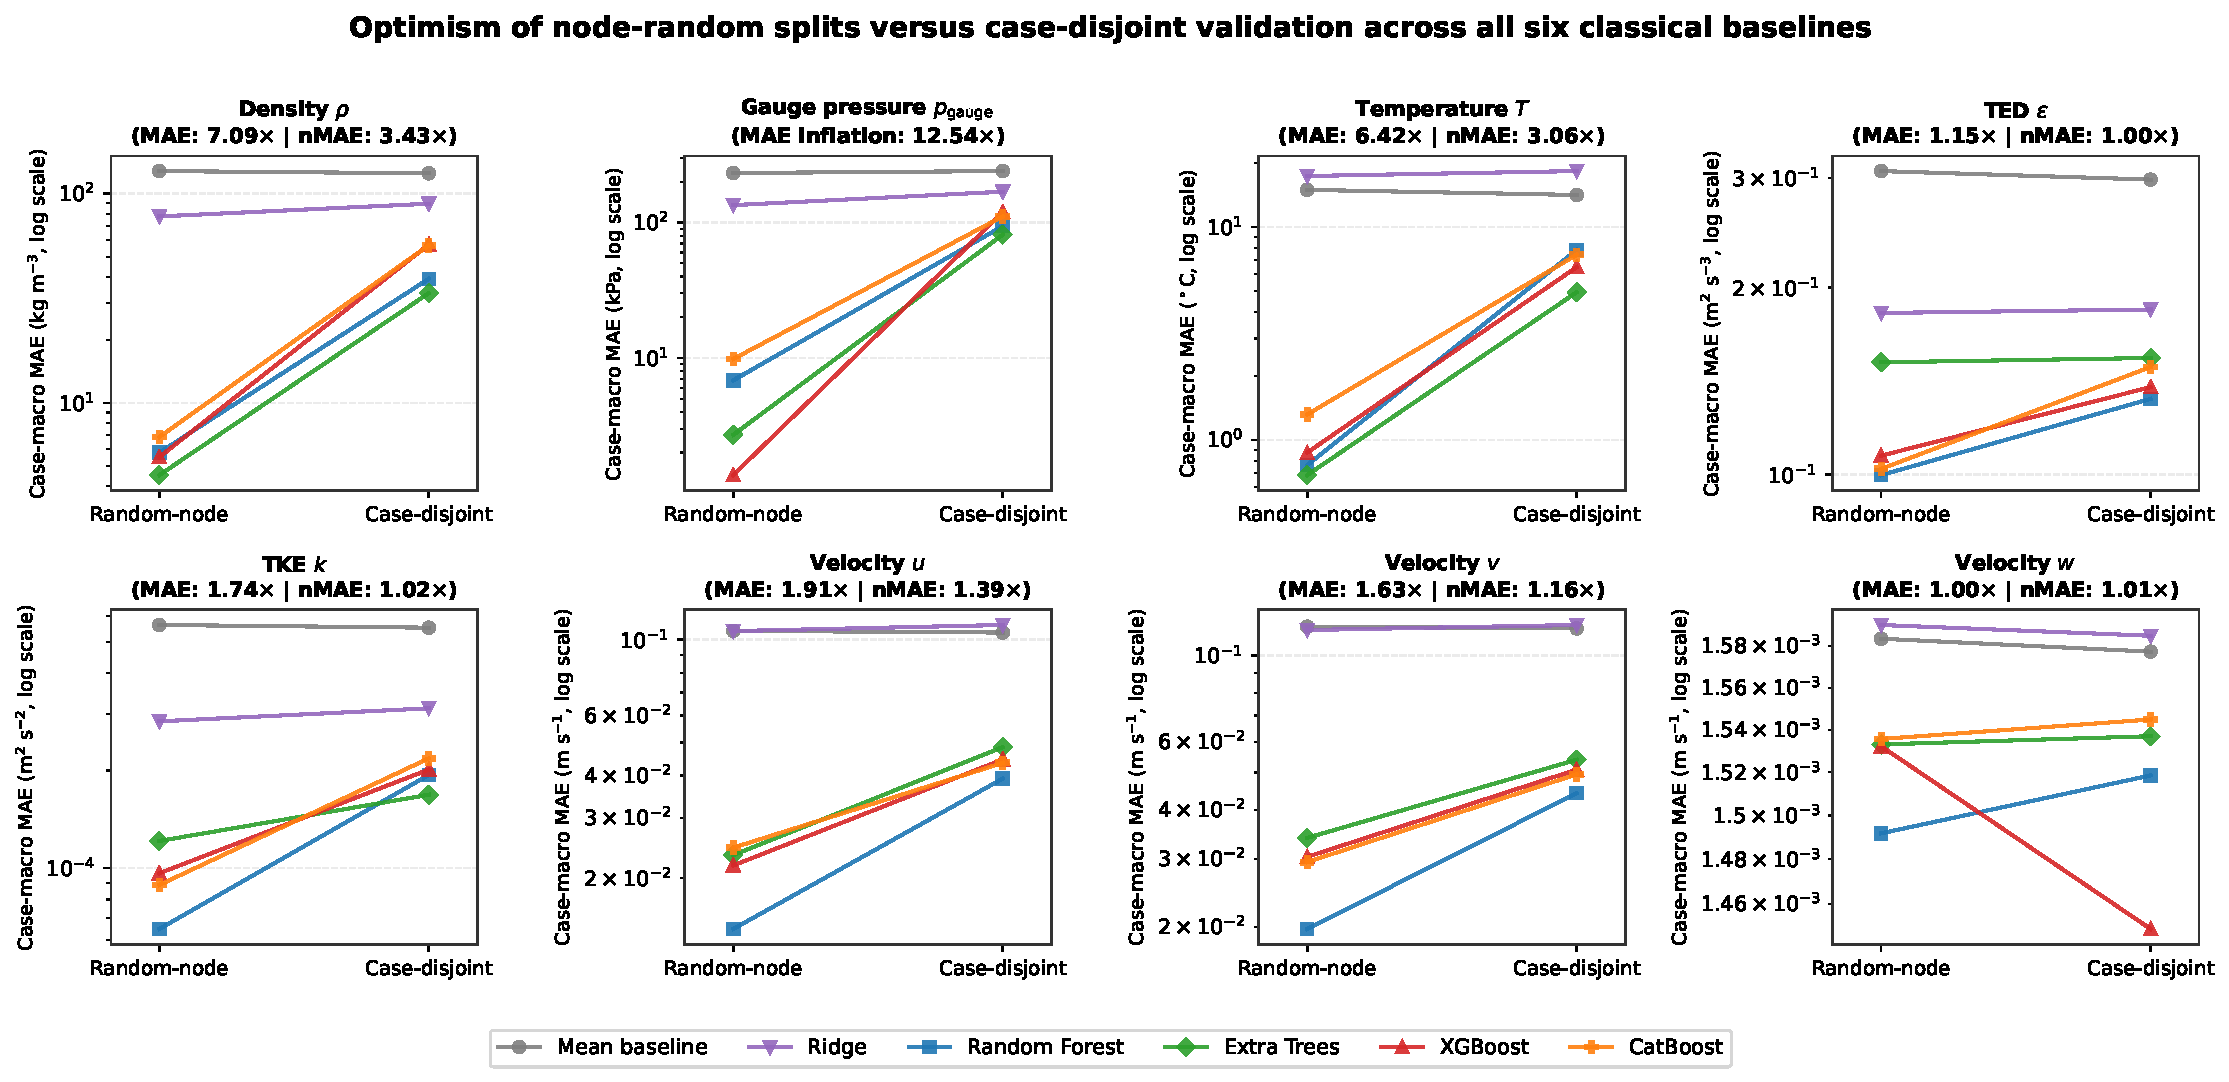
\includegraphics[width=1.00\textwidth]{random_node_vs_case_disjoint_nmae.pdf}
\caption{Case-macro MAE (log scale) under 80/20 random-node splits versus five-fold case-disjoint validation across the four nonlinear tree baselines (\texttt{RF}, \texttt{ET}, \texttt{XGB}, \texttt{CB}) and two controls (\texttt{Mean}, \texttt{Ridge}).}
\label{fig:leakage}
\end{figure}

\subsection{Three-Seed Case-Disjoint Benchmark Across All Eight CFD Fields}
Figure~\ref{fig:heatmap} shows the three-seed (\texttt{2026}, \texttt{2027}, \texttt{2028}) case-macro MAE of all 18 models relative to the \texttt{Mean baseline}, and Table~\ref{tab:main} reports the detailed metrics of the top-performing pooled and within-group models for each field (complete 19-model tables are in Supplementary Tables~S1--S8).

\begin{figure}[!htbp]
\centering
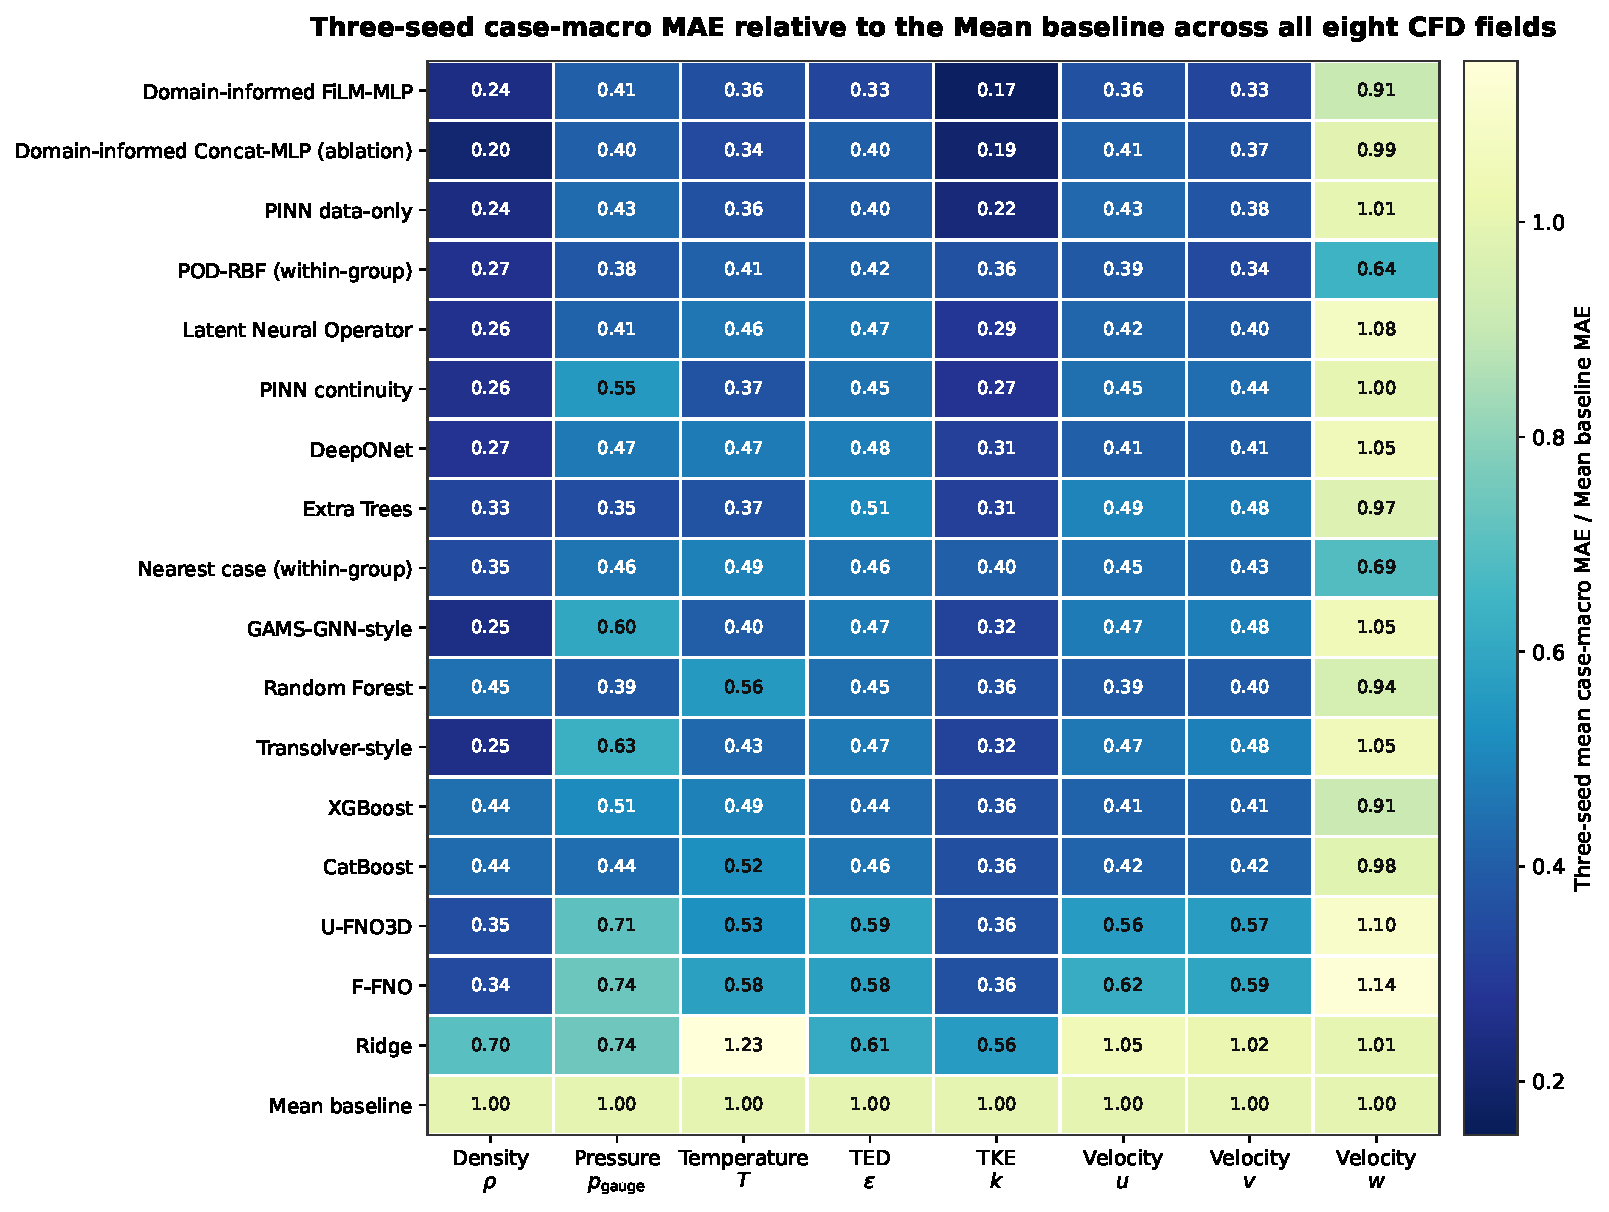
\includegraphics[width=0.98\textwidth]{final_three_seed_error_ratio_heatmap.pdf}
\caption{Three-seed mean case-macro MAE relative to the \texttt{Mean baseline} across all eight CFD fields, ordered by geometric-mean relative error.}
\label{fig:heatmap}
\end{figure}

\begin{table}[!htbp]
\centering
\caption{Three-seed (\texttt{2026}, \texttt{2027}, \texttt{2028}) out-of-fold accuracy across the 42 $\mathrm{sCO}_2$ cases. For each target, the leading cross-configuration pooled model is listed first, followed by the best within-group mesh-aligned model where it achieves lower error (and the lowest-MAE pooled model on $\rho$).}
\label{tab:main}
\small
\setlength{\tabcolsep}{4.8pt}
\begin{tabular}{llrrrrrrr}
\toprule
Target & Model & Scope & Macro & Mean-base & Reduction & Macro & Median nMAE & Pooled \\
(unit) & & & MAE & MAE & (\%) & RMSE & ($\pm$SD) & $R^2$ \\
\midrule
$\rho$ (kg m$^{-3}$) & \texttt{DeepONet} & Pooled & 35.1 & 131.6 & 73.3\% & 37.1 & $0.837 \pm 0.160$ & 0.862 \\
 & \texttt{Concat-MLP} & Pooled & 26.3 & 131.6 & 80.0\% & 29.1 & $1.011 \pm 0.069$ & 0.936 \\
\midrule
$p_{\mathrm{gauge}}$ (kPa) & \texttt{Extra Trees} & Pooled & 83.2 & 254.0 & 67.3\% & 83.7 & $2.91^\dagger$ & 0.815 \\
 & \texttt{POD-RBF} & Aligned & 90.1 & 254.0 & 64.5\% & 90.2 & $0.0483^\dagger$ & 0.571 \\
 & \texttt{Nearest case} & Aligned & 108.1 & 254.0 & 57.4\% & 108.2 & $0.0122^\dagger$ & 0.776 \\
\midrule
$T$ ($^\circ$C) & \texttt{PINN continuity} & Pooled & 5.48 & 13.71 & 60.0\% & 7.32 & $1.350 \pm 0.044$ & 0.736 \\
 & \texttt{POD-RBF} & Aligned & 6.11 & 13.71 & 55.4\% & 7.42 & $0.974 \pm 0.041$ & 0.620 \\
\midrule
$\varepsilon$ (m$^2$ s$^{-3}$) & \texttt{FiLM-MLP} & Pooled & 0.0978 & 0.1945 & 49.7\% & 0.315 & $0.192 \pm 0.020$ & 0.569 \\
 & \texttt{POD-RBF} & Aligned & 0.127 & 0.1945 & 34.8\% & 0.369 & $0.177 \pm 0.018$ & $-0.575$ \\
\midrule
$k$ ($10^{-4}$ m$^2$ s$^{-2}$) & \texttt{FiLM-MLP} & Pooled & 0.947 & 3.635 & 73.9\% & 1.57 & $0.242 \pm 0.051$ & 0.898 \\
 & \texttt{POD-RBF} & Aligned & 2.00 & 3.635 & 45.0\% & 2.78 & $0.237 \pm 0.015$ & $-0.070$ \\
\midrule
$u$ (m s$^{-1}$) & \texttt{FiLM-MLP} & Pooled & 0.0381 & 0.1763 & 78.4\% & 0.0569 & $0.162 \pm 0.015$ & 0.801 \\
$v$ (m s$^{-1}$) & \texttt{FiLM-MLP} & Pooled & 0.0383 & 0.1972 & 80.6\% & 0.0591 & $0.175 \pm 0.004$ & 0.861 \\
\midrule
$w$ ($10^{-3}$ m s$^{-1}$) & \texttt{FiLM-MLP} & Pooled & 1.43 & 2.660 & 46.3\% & 3.46 & $0.272 \pm 0.007$ & 0.418 \\
 & \texttt{POD-RBF} & Aligned & 1.01 & 2.660 & 62.1\% & 2.55 & $0.207 \pm 0.008$ & 0.650 \\
 & \texttt{Nearest case} & Aligned & 1.08 & 2.660 & 59.3\% & 2.93 & $0.185 \pm 0.009$ & 0.551 \\
\bottomrule
\end{tabular}
\begin{flushleft}\footnotesize $^\dagger$ For gauge pressure, the Median nMAE column reports the centered spatial residual $\mathrm{nRMSE}_{\mathrm{res}}$ ($1\text{ kPa}$ floor; Table~S8).\end{flushleft}
\end{table}

Four main findings emerge from Table~\ref{tab:main} and Figure~\ref{fig:heatmap}:
\begin{enumerate}
  \item \textbf{State fields ($\rho, T$) vs.\ kinematic/turbulence fields ($u, v, w, k, \varepsilon$):} On density and temperature, pooled models reduce case-macro MAE by $73.3\%\text{--}80.0\%$ ($\rho$) and $60.0\%$ ($T$) and reach high pooled $R^2$ ($0.862\text{--}0.936$ and $0.736$), but narrow within-case standard deviations in the small loops ($\sigma_c(T) \approx 0.25\text{--}2.5^\circ\text{C}$) keep median case nMAE at $0.837$ (\texttt{DeepONet} on $\rho$) and $1.350$ (\texttt{PINN continuity} on $T$; reduced to $0.974$ by within-group \texttt{POD-RBF}). Conversely, velocity and turbulence fields have near-zero case-mean offsets and strong geometry-locked spatial profiles; here \texttt{Domain-informed FiLM-MLP} achieves median case nMAE of $0.162$ ($u$), $0.175$ ($v$), $0.192$ ($\varepsilon$), and $0.242$ ($k$).
  \item \textbf{FiLM modulation vs.\ input concatenation:} Relative to \texttt{Domain-informed Concat-MLP}, multiplicative FiLM conditioning reduces median case nMAE on six of the seven spatially varying fields: $T$ ($1.467$ vs.\ $1.758$), $\varepsilon$ ($0.192$ vs.\ $0.226$), $k$ ($0.242$ vs.\ $0.273$), $u$ ($0.162$ vs.\ $0.224$), $v$ ($0.175$ vs.\ $0.230$), and $w$ ($0.272$ vs.\ $0.318$), whereas concatenation yields lower case-macro MAE on density ($26.3$ vs.\ $31.3\text{ kg m}^{-3}$).
  \item \textbf{Gauge-pressure level vs.\ spatial residual:} Total gauge-pressure MAE ($83.2\text{ kPa}$ for \texttt{Extra Trees}, a $67.3\%$ reduction below the \texttt{Mean baseline}) is dominated by the case-level offset $e_{\mathrm{level},c}$ ($82.9\text{ kPa}$). On the centered spatial residual $\tilde{p}_{c,i}$ (Supplementary Table~S8), mesh-aligned \texttt{Nearest case} ($\mathrm{nRMSE}_{\mathrm{res}} = 0.0122$), \texttt{POD-GPR} ($0.0457$), \texttt{POD-RBF} ($0.0483$), and \texttt{XGBoost} ($0.151$) preserve the smooth hydrostatic profile, whereas coordinate networks exhibit higher residual roughness ($\mathrm{nRMSE}_{\mathrm{res}} = 2.91\text{--}24.3$).
  \item \textbf{Voxelized FNOs on slender pipe loops:} \texttt{F-FNO} and \texttt{U-FNO3D} rank near the bottom of the neural models (Fig.~\ref{fig:heatmap}) because voxelizing thin pipes ($D_i/L < 1.7\%$) onto a $64\times 64\times 16$ Cartesian grid places only 1--2 cells across the pipe diameter, blurring radial boundary-layer gradients.
\end{enumerate}

\noindent\textbf{Exploratory statistical comparisons:} Treating nonparametric Friedman tests and Holm-adjusted two-sided Wilcoxon signed-rank tests across the 42 cases (three-seed mean five-fold errors; Supplementary Table~S10) as exploratory, overall model differences are significant on all eight fields ($p < 0.001$). Against \texttt{Domain-informed FiLM-MLP} ($\alpha = 0.05$): (i) on $\varepsilon$ and $k$, \texttt{FiLM-MLP} ranks first (mean rank $4.62$), significantly outperforming all 15 pooled baselines on $\varepsilon$ and 14 of 15 on $k$ (all except \texttt{Concat-MLP}, $p_{\mathrm{Holm}} = 0.190$), while not differing significantly from within-group \texttt{POD-RBF}, \texttt{POD-GPR}, and \texttt{Nearest case} ($p_{\mathrm{Holm}} \ge 0.190$); (ii) on $u$ and $v$, \texttt{FiLM-MLP} ranks first ($5.83$ and $5.26$), significantly outperforming \texttt{Concat-MLP}, both \texttt{PINNs}, \texttt{LNO}, \texttt{Transolver-style}, \texttt{GAMS-GNN-style}, both \texttt{FNOs}, \texttt{Ridge}, and \texttt{Mean baseline} ($p_{\mathrm{Holm}} < 0.05$, plus \texttt{DeepONet} and \texttt{Extra Trees} on $v$), while not differing significantly from the remaining tree ensembles or within-group aligned models ($p_{\mathrm{Holm}} \ge 0.052$); (iii) on $w$, \texttt{FiLM-MLP} is significantly outperformed by within-group \texttt{POD-RBF}, \texttt{POD-GPR}, and \texttt{Nearest case}, does not differ significantly from \texttt{PINN continuity}, tree ensembles, \texttt{Ridge}, or \texttt{Mean baseline} ($p_{\mathrm{Holm}} \ge 0.096$), and significantly outperforms all other neural/operator baselines ($p_{\mathrm{Holm}} < 0.05$); and (iv) on $\rho$ and $T$, \texttt{FiLM-MLP} is significantly outperformed by \texttt{POD-RBF} on $T$, does not differ significantly from \texttt{DeepONet}, \texttt{Concat-MLP}, \texttt{PINNs}, \texttt{Transolver-style}, \texttt{GAMS-GNN-style}, or \texttt{Extra Trees} ($p_{\mathrm{Holm}} \ge 0.170$), and significantly outperforms \texttt{F-FNO}, \texttt{U-FNO3D}, \texttt{Ridge}, and \texttt{Mean baseline} (plus \texttt{RF}, \texttt{XGB}, \texttt{CB}, and \texttt{POD-GPR} on $\rho$, and \texttt{LNO} on $T$).

\subsection{Spatial Reconstruction Analysis and Leave-One-Group-Out Extrapolation}
Figure~\ref{fig:maps} shows held-out CFD fields, surrogate predictions, and absolute error maps (seed \texttt{2026}, labeled by $\mathrm{nMAE}_c$ rank) for showcase cases on $\rho$ (\texttt{DeepONet}, rank $15/42$; 3-seed rank $3/42$), $T$ (\texttt{PINN continuity}, rank $17/42$; 3-seed rank $1/42$), and $v$ (\texttt{FiLM-MLP}, rank $10/42$; 3-seed rank $3/42$). Supplementary Figure~S1 shows the corresponding \textbf{median (rank 21/42)} and \textbf{worst (rank 42/42)} held-out cases per field: median cases accurately capture loop-scale stratification and riser/downcomer velocity cores with errors localized near the cooler wall and elbows, whereas rank-42/42 cases occur at extreme boundary conditions (\texttt{HHHC\_P2000\_90\_bar\_0.05kgs\_T\_315} on $\rho$ and $T$, the sole case with $T_{\mathrm{in}}=315\text{ K}$ and $\bar{T}_c = 47.5^\circ\text{C}$) or in the near-stagnant \texttt{HHVC\_P20\_90\_bar\_0.05kgs\_T\_305} run on $v$ ($\sigma_c(v) = 1.5\text{ mm s}^{-1}$).

\begin{figure}[!htbp]
\centering
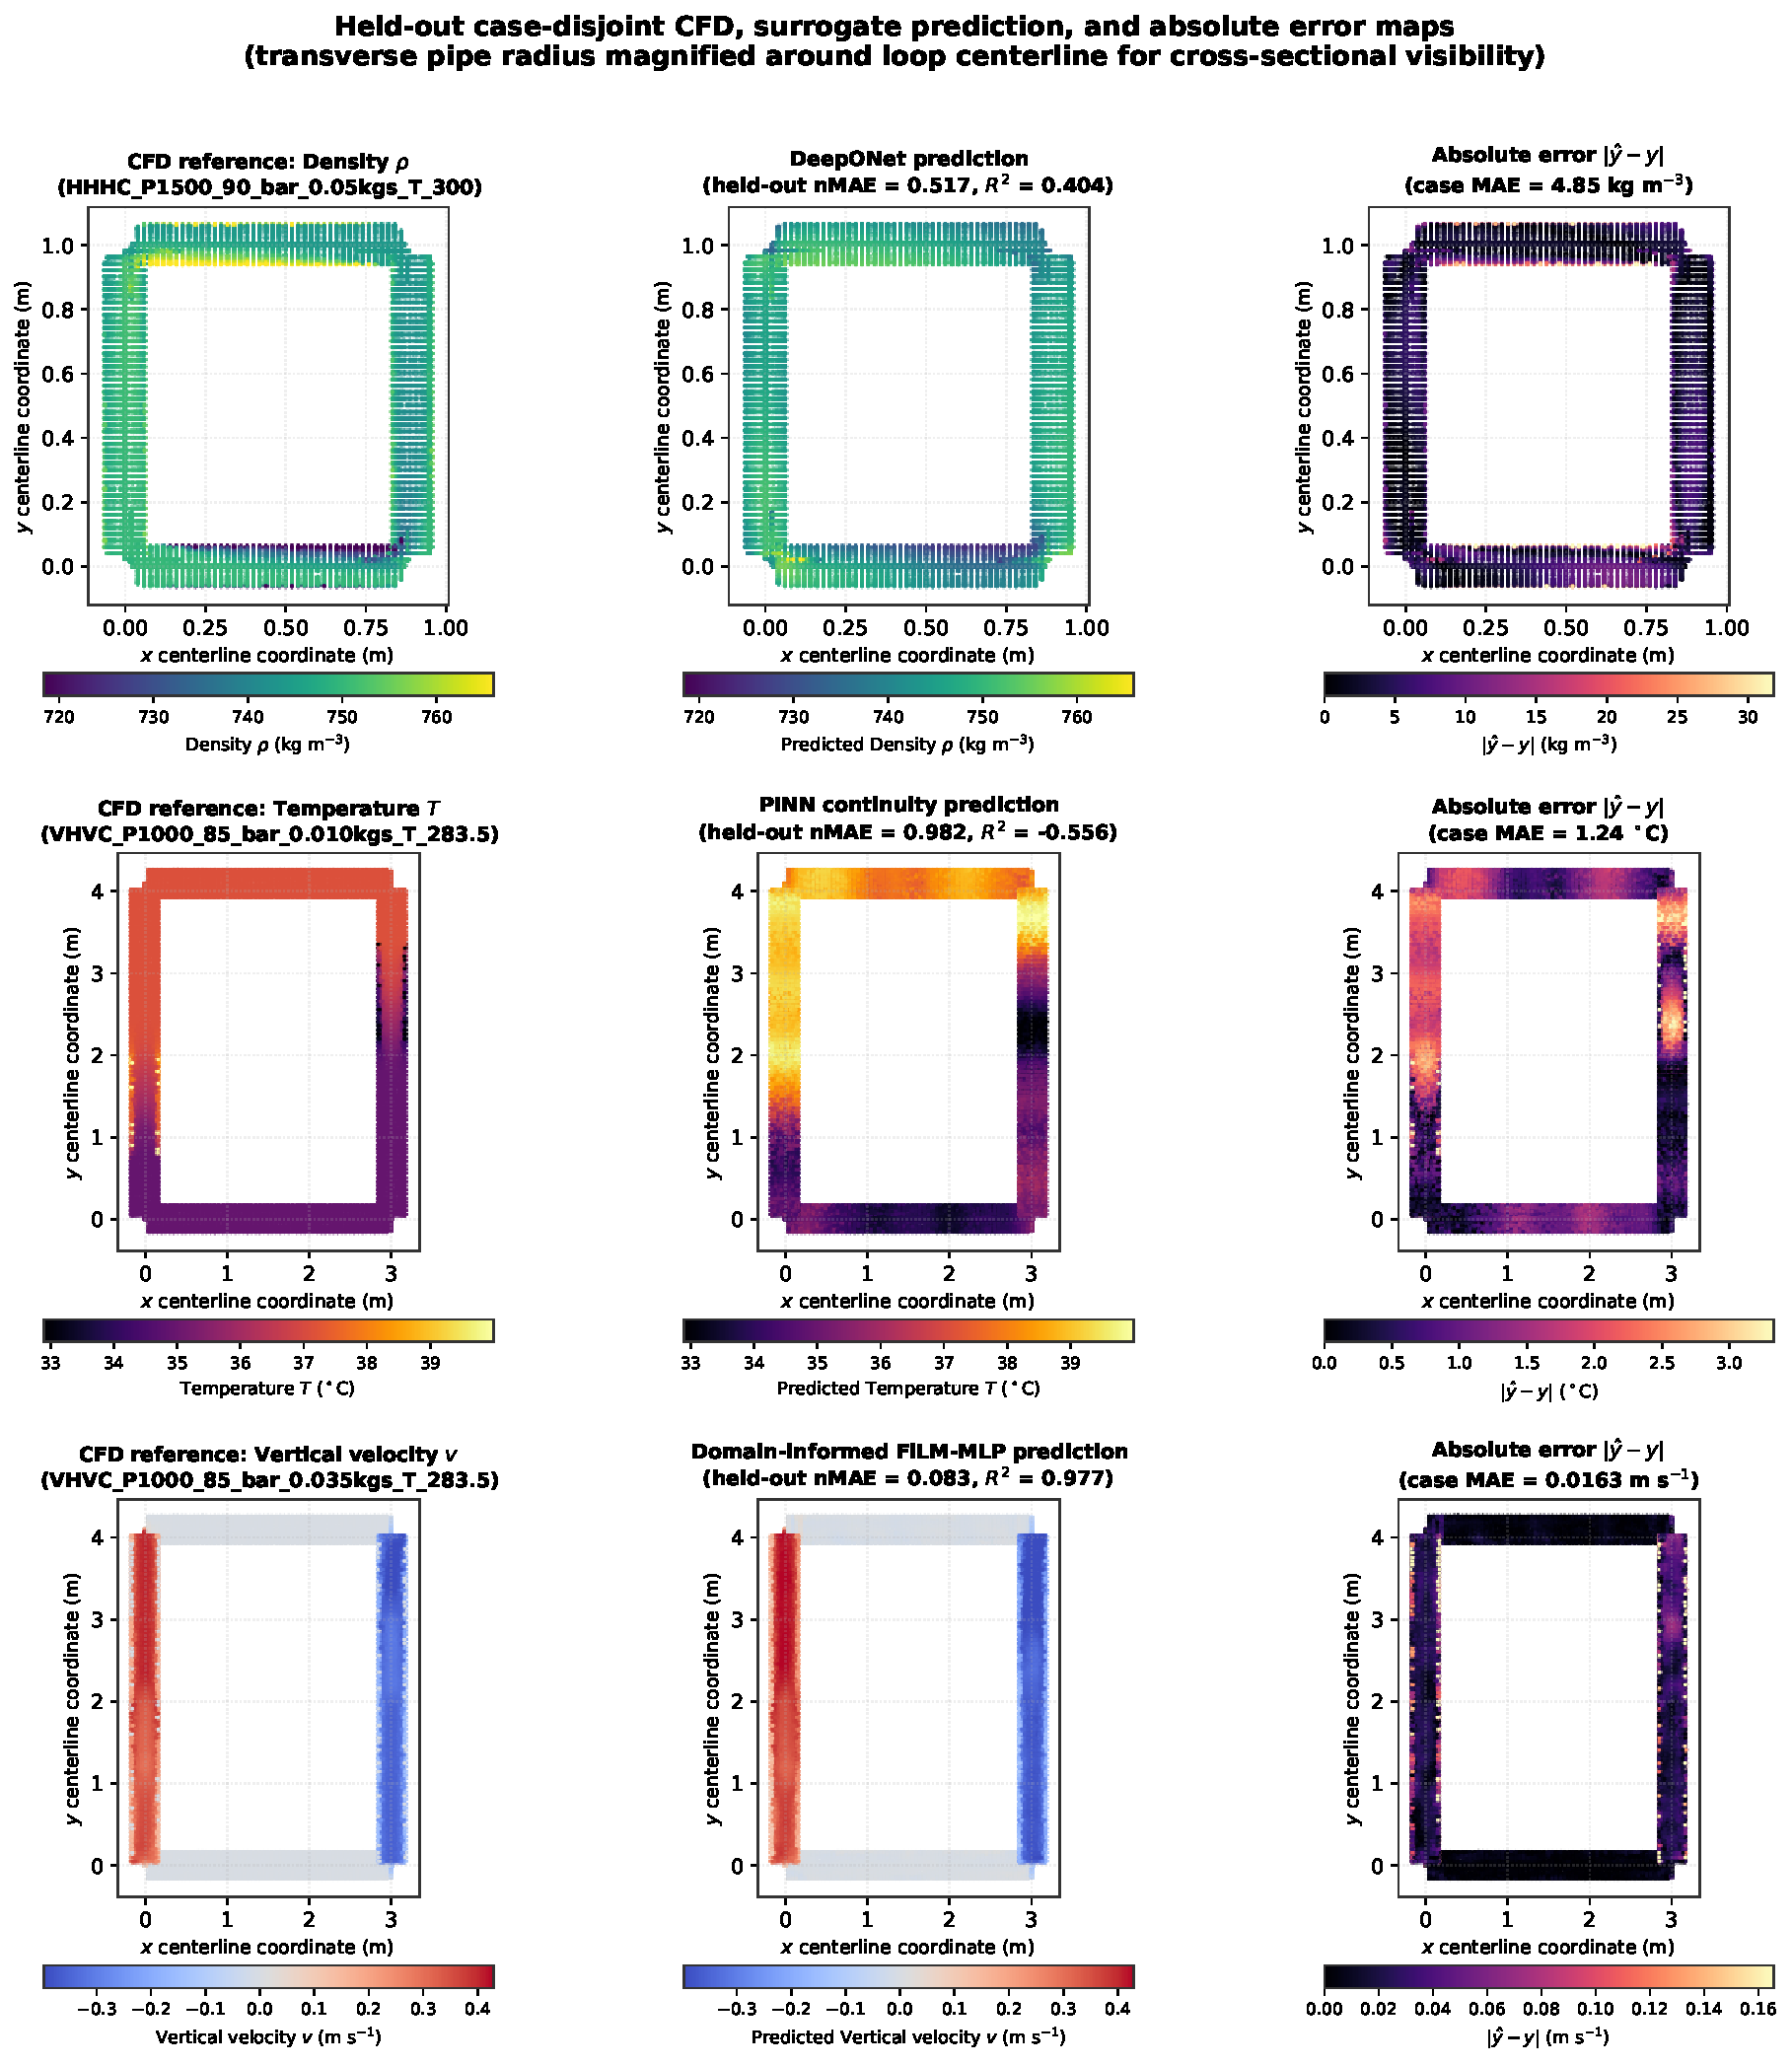
\includegraphics[width=1.00\textwidth,height=0.84\textheight,keepaspectratio]{heldout_cfd_prediction_error_maps.pdf}
\caption{Held-out out-of-fold spatial reconstructions (seed \texttt{2026}) comparing reference CFD (left), surrogate prediction (middle), and absolute error $|\hat{y}-y|$ (right) for $\rho$ (\texttt{DeepONet}, rank $15/42$), $T$ (\texttt{PINN continuity}, rank $17/42$), and $v$ (\texttt{Domain-informed FiLM-MLP}, rank $10/42$). Median (rank $21/42$) and worst (rank $42/42$) cases per field are shown in Supplementary Figure~S1.}
\label{fig:maps}
\end{figure}

Table~\ref{tab:groupholdout} summarizes the leave-one-group-out extrapolation study across the four structural groups ($16\text{ pooled models} \times 8\text{ fields} = 128$ model--field evaluations per group; full metrics in Supplementary Table~S9). When \texttt{VHVC/small} ($n=4$) is held out, both the small-loop geometry ($0.894\times 1.000\text{ m}$, $90\text{ bar}$, $305\text{ K}$) and the \texttt{VHVC} orientation have been seen during training, allowing \texttt{XGBoost} and \texttt{FiLM-MLP} to maintain moderate median nMAE ($\rho$: $0.980$, $T$: $1.609$, $\varepsilon$: $0.268$, $k$: $0.391$, $v$: $0.686$). Conversely, holding out \texttt{VHVC/large} ($n=13$) or \texttt{HHHC/small} ($n=20$) requires extrapolating across an unseen loop scale ($3.010\times 4.080\text{ m}$, $D_i = 13.84\text{ mm}$, $T_{\mathrm{in}} = 283.5\text{ K}$) or an unseen top-horizontal cooler configuration ($Q = 1000\text{--}2000\text{ W}$), inflating the best density median nMAE to $3.854$ and $4.601$.

\begin{table}[!htbp]
\centering
\caption{Leave-one-group-out extrapolation summary across the four structural groups. Each cell reports the winning pooled model and its three-seed mean median case nMAE across the $16\text{ models}\times 8\text{ fields} = 128$ evaluations per group ($p_{\mathrm{gauge}}$ is reported via level MAE and residual $\mathrm{nRMSE}_{\mathrm{res}}$).}
\label{tab:groupholdout}
\small
\setlength{\tabcolsep}{3.8pt}
\begin{tabular}{lllll}
\toprule
Field & \texttt{HHHC/small} ($n=20$) & \texttt{HHVC/small} ($n=5$) & \texttt{VHVC/small} ($n=4$) & \texttt{VHVC/large} ($n=13$) \\
\midrule
$\rho$ (nMAE) & \texttt{PINN cont.} ($4.601$) & \texttt{PINN data} ($21.13$) & \texttt{XGBoost} ($0.980$) & \texttt{Random Forest} ($3.854$) \\
$T$ (nMAE) & \texttt{PINN cont.} ($9.572$) & \texttt{PINN data} ($11.53$) & \texttt{XGBoost} ($1.609$) & \texttt{PINN data} ($1.682$) \\
$\varepsilon$ (nMAE) & \texttt{Transolver} ($0.464$) & \texttt{Concat-MLP} ($0.822$) & \texttt{FiLM-MLP} ($0.268$) & \texttt{GAMS-GNN} ($0.258$) \\
$k$ (nMAE) & \texttt{Concat-MLP} ($1.198$) & \texttt{Concat-MLP} ($1.242$) & \texttt{FiLM-MLP} ($0.391$) & \texttt{GAMS-GNN} ($0.752$) \\
$u$ (nMAE) & \texttt{Extra Trees} ($0.710$) & \texttt{Mean base.} ($0.869$) & \texttt{Mean base.} ($0.875$) & \texttt{Concat-MLP} ($0.810$) \\
$v$ (nMAE) & \texttt{XGBoost} ($0.733$) & \texttt{Mean base.} ($0.873$) & \texttt{XGBoost} ($0.686$) & \texttt{Concat-MLP} ($0.766$) \\
$w$ (nMAE) & \texttt{Transolver} ($0.687$) & \texttt{Mean base.} ($0.736$) & \texttt{GAMS-GNN} ($0.692$) & \texttt{Mean base.} ($0.558$) \\
\midrule
$p_{\mathrm{gauge}}$ level MAE (kPa) & \texttt{DeepONet} ($254.0$) & \texttt{Mean base.} ($536.2$) & \texttt{F-FNO} ($226.4$) & \texttt{Ridge} ($204.2$) \\
$p_{\mathrm{gauge}}$ res.\ $\mathrm{nRMSE}_{\mathrm{res}}$ & \texttt{Mean base.} ($0.273$) & \texttt{Mean base.} ($0.197$) & \texttt{Mean base.} ($0.172$) & \texttt{Extra Trees} ($0.734$) \\
\bottomrule
\end{tabular}
\end{table}

\subsection{Limitations}
Three limitations of this study should be noted: (1) because only final converged CFD-Post exports are available without solver convergence histories, we cannot separate a physical flow-regime transition from convergence to an alternative steady numerical branch in the two near-stagnant cases \texttt{HHVC\_P20\_90\_bar\_0.05kgs\_T\_305} ($Q=20\text{ W}$) and \texttt{HHVC\_P30\_90\_bar\_0.05kgs\_T\_305} ($Q=30\text{ W}$), nor can we verify the specific $k$--$\varepsilon$ sub-variant, wall-function treatment, or unexported hydrostatic reference density $\rho_0$; (2) plane-weighted mean $\mathrm{CO}_2$ density $\bar{\rho}_{\mathrm{plane},c}$ varies across steady-state cases at the same $(p_{\mathrm{op}}, T_{\mathrm{in}})$ (Section~2.2), so the cases represent independent steady runs rather than a strictly constant-mass trajectory; and (3) seeds \texttt{2026}, \texttt{2027}, and \texttt{2028} re-randomize the five-fold stratified case splits in addition to model initialization, and the small group sizes in \texttt{HHVC/small} ($n=5$) and \texttt{VHVC/small} ($n=4$) limit statistical power under group holdout.

\section{Conclusions}
We have presented a case-disjoint surrogate benchmark across 42 steady-state $\mathrm{sCO}_2$ natural-circulation loop CFD simulations ($5,451,341$ primary $\mathrm{sCO}_2$ nodes). Our main conclusions are:
\begin{enumerate}
  \item \textbf{Case-disjoint validation and two-part pressure evaluation are essential:} Across the four nonlinear tree baselines, 80/20 random node splits understate five-fold case-disjoint case-macro MAE by $6.78\times\text{--}10.37\times$ on density, $11.29\times\text{--}87.54\times$ on gauge pressure, and $5.62\times\text{--}10.24\times$ on temperature ($3.34\times\text{--}4.05\times$ and $2.95\times\text{--}4.39\times$ in median case nMAE on $\rho$ and $T$), while \texttt{Mean} and \texttt{Ridge} controls remain near $1.0\times\text{--}1.26\times$. Separating gauge pressure into its case-level mean offset and centered spatial residual prevents between-case pressurization shifts from obscuring within-loop gradient accuracy.
  \item \textbf{Different physical fields favor distinct inductive biases:} Under three-seed five-fold case-disjoint cross-validation, multiplicative coordinate modulation (\texttt{Domain-informed FiLM-MLP}) leads all pooled models across all three velocity components ($\mathrm{nMAE} = 0.162, 0.175, 0.272$) and both turbulence fields ($\mathrm{nMAE} = 0.192$ on $\varepsilon$, $0.242$ on $k$); \texttt{DeepONet} ($\mathrm{nMAE} = 0.837$) and \texttt{PINN continuity} ($\mathrm{nMAE} = 1.350$) lead among pooled models on density and temperature; and within-group \texttt{POD-RBF} achieves the lowest within-case nMAE on temperature ($0.974$), $\varepsilon$ ($0.177$), and $k$ ($0.237$) when interpolating on a fixed mesh, whereas uniform voxelized spectral operators (\texttt{F-FNO}, \texttt{U-FNO}) underperform on slender pipe geometries ($D_i/L < 1.7\%$).
  \item \textbf{Cross-geometry extrapolation requires multi-scale coverage:} Leave-one-group-out tests ($128$ model--field evaluations per group) show that pooled models transfer across heater orientations when the loop scale is covered in training (\texttt{VHVC/small}), but degrade when extrapolating across a $3.4\times\text{--}4.1\times$ change in loop dimensions and operating regime (\texttt{VHVC/large}, \texttt{HHHC/small}).
\end{enumerate}

\section*{Data and Code Availability}
All preprocessing, benchmark training, statistical testing, and plotting scripts, along with the three-seed metric tables, pressure/density audit CSV, and supplementary material (Section~S1, Figure~S1, and Tables~S0a--S10), are publicly available at \url{\repourl}.

\begin{thebibliography}{99}\small\setlength{\itemsep}{1pt}\setlength{\parskip}{0pt}

\bibitem{swapnalee2012generalized}
B.~T. Swapnalee, P.~K. Vijayan, M.~Sharma, and D.~S. Pilkhwal, ``Steady state flow and static instability of supercritical natural circulation loops,'' \emph{Nuclear Engineering and Design}, vol.~245, pp.~99--112, 2012, doi:10.1016/j.nucengdes.2012.01.002.

\bibitem{vijayan2002experimental}
P.~K. Vijayan, ``Experimental observations on the general trends of the steady state and stability behaviour of single-phase natural circulation loops,'' \emph{Nuclear Engineering and Design}, vol.~215, no.~1--2, pp.~139--152, 2002, doi:10.1016/S0029-5493(02)00047-X.

\bibitem{pioro2007heat}
I.~L. Pioro and R.~B. Duffey, \emph{Heat Transfer and Hydraulic Resistance at Supercritical Pressures in Power Engineering Applications}. New York, NY, USA: ASME Press, 2007, doi:10.1115/1.802526.

\bibitem{span1996new}
R.~Span and W.~Wagner, ``A new equation of state for carbon dioxide covering the fluid region from the triple-point temperature to 1100 K at pressures up to 800 MPa,'' \emph{Journal of Physical and Chemical Reference Data}, vol.~25, no.~6, pp.~1509--1596, 1996, doi:10.1063/1.555991.

\bibitem{dostal2004supercritical}
V.~Dostal, M.~J. Driscoll, and P.~Hejzlar, ``A supercritical carbon dioxide cycle for next generation nuclear reactors,'' MIT Center for Advanced Nuclear Energy Systems, Cambridge, MA, USA, Tech. Rep. MIT-ANP-TR-100, 2004.

\bibitem{bae2005mixed}
J.~H. Bae, J.~Y. Yoo, and H.~Choi, ``Direct numerical simulation of turbulent supercritical flows with heat transfer,'' \emph{Physics of Fluids}, vol.~17, no.~10, p.~105104, 2005, doi:10.1063/1.2047588.

\bibitem{kurganov2013heat}
V.~A. Kurganov, Y.~A. Zeigarnik, and I.~V. Maslakova, ``Heat transfer and hydraulic resistance of supercritical pressure fluids in circular tubes under heating conditions,'' \emph{International Journal of Heat and Mass Transfer}, vol.~58, no.~1--2, pp.~152--167, 2013, doi:10.1016/j.ijheatmasstransfer.2012.10.072.

\bibitem{sarkar2014entropy}
M.~K.~S. Sarkar, D.~N. Basu, and P.~K. Das, ``Thermalhydraulic characteristics of supercritical natural circulation loops: A review,'' \emph{Nuclear Engineering and Design}, vol.~274, pp.~155--175, 2014, doi:10.1016/j.nucengdes.2014.04.011.

\bibitem{chen2013numerical}
L.~Chen, B.-L. Deng, B.~Jiang, and X.-R. Zhang, ``Numerical and experimental investigation of natural convection loop with supercritical $\mathrm{CO}_2$,'' \emph{International Journal of Heat and Mass Transfer}, vol.~64, pp.~202--214, 2013, doi:10.1016/j.ijheatmasstransfer.2013.03.077.

\bibitem{friedman2001greedy}
J.~H. Friedman, ``Greedy function approximation: A gradient boosting machine,'' \emph{The Annals of Statistics}, vol.~29, no.~5, pp.~1189--1232, 2001, doi:10.1214/aos/1013203451.

\bibitem{chen2016xgboost}
T.~Chen and C.~Guestrin, ``XGBoost: A scalable tree boosting system,'' in \emph{Proceedings of the 22nd ACM SIGKDD International Conference on Knowledge Discovery and Data Mining}, 2016, pp.~785--794, doi:10.1145/2939672.2939785.

\bibitem{prokhorenkova2018catboost}
L.~Prokhorenkova, G.~Gusev, A.~Vorobev, A.~V. Dorogush, and A.~Gulin, ``CatBoost: Unbiased boosting with categorical features,'' in \emph{Advances in Neural Information Processing Systems (NeurIPS)}, vol.~31, 2018, pp.~6638--6648.

\bibitem{raissi2019physics}
M.~Raissi, P.~Perdikaris, and G.~E. Karniadakis, ``Physics-informed neural networks: A deep learning framework for solving forward and inverse problems involving nonlinear partial differential equations,'' \emph{Journal of Computational Physics}, vol.~378, pp.~686--707, 2019, doi:10.1016/j.jcp.2018.10.045.

\bibitem{tancik2020fourier}
M.~Tancik, P.~Srinivasan, B.~Mildenhall, S.~Fridovich-Keil, N.~Raghavan, U.~Singhal, R.~Ramamoorthi, J.~Barron, and R.~Ng, ``Fourier features let networks learn high frequency functions in low dimensional domains,'' in \emph{Advances in Neural Information Processing Systems (NeurIPS)}, vol.~33, 2020, pp.~7537--7547.

\bibitem{perez2018film}
E.~Perez, F.~Strub, H.~de~Vries, V.~Dumoulin, and A.~Courville, ``FiLM: Visual reasoning with a general conditioning layer,'' in \emph{Proceedings of the AAAI Conference on Artificial Intelligence}, vol.~32, no.~1, 2018, pp.~3942--3951, doi:10.1609/aaai.v32i1.11671.

\bibitem{lu2021learning}
L.~Lu, P.~Jin, G.~Pang, Z.~Zhang, and G.~E. Karniadakis, ``Learning nonlinear operators via DeepONet based on the universal approximation theorem of operators,'' \emph{Nature Machine Intelligence}, vol.~3, no.~3, pp.~218--229, 2021, doi:10.1038/s42256-021-00302-5.

\bibitem{li2021fourier}
Z.~Li, N.~Kovachki, K.~Azizzadenesheli, B.~Liu, K.~Bhattacharya, A.~Stuart, and A.~Anandkumar, ``Fourier neural operator for parametric partial differential equations,'' in \emph{International Conference on Learning Representations (ICLR)}, 2021.

\bibitem{wen2022ufno}
G.~Wen, Z.~Li, K.~Azizzadenesheli, A.~Anandkumar, and S.~M. Benson, ``U-FNO---An enhanced Fourier neural operator-based deep-learning model for multiphase flow,'' \emph{Advances in Water Resources}, vol.~163, p.~104180, 2022, doi:10.1016/j.advwatres.2022.104180.

\bibitem{wu2024transolver}
H.~Wu, H.~Luo, H.~Wang, J.~Wang, and M.~Long, ``Transolver: A fast transformer solver for PDEs on general geometries,'' in \emph{Proceedings of the 41st International Conference on Machine Learning (ICML)}, vol.~235, 2024, pp.~53681--53705.

\bibitem{berkooz1993proper}
G.~Berkooz, P.~Holmes, and J.~L. Lumley, ``The proper orthogonal decomposition in the analysis of turbulent flows,'' \emph{Annual Review of Fluid Mechanics}, vol.~25, no.~1, pp.~539--575, 1993, doi:10.1146/annurev.fl.25.010193.002543.

\bibitem{audouze2009nonintrusive}
C.~Audouze, F.~De~Vuyst, and P.~B. Nair, ``Nonintrusive reduced-order modeling of parametrized time-dependent partial differential equations,'' \emph{Numerical Methods for Partial Differential Equations}, vol.~29, no.~5, pp.~1587--1628, 2013, doi:10.1002/num.21768.

\bibitem{bell2014pure}
I.~H. Bell, J.~Wronski, S.~Quoilin, and V.~Lemort, ``Pure and pseudo-pure fluid thermophysical property evaluation and the open-source thermophysical property library CoolProp,'' \emph{Industrial \& Engineering Chemistry Research}, vol.~53, no.~6, pp.~2498--2508, 2014, doi:10.1021/ie4033999.

\end{thebibliography}

\end{document}
